% -------------------------------------------------------------
% --------------------- LECTURE 12 4-6/12 ---------------------
% -------------------------------------------------------------
% flipped classroom

\chapter{Classification of topological field theories}\label{ClassificationOfTFTs}
\epigraph{
\textbf{Existence}: Why is there something, rather than nothing?

\noindent This does not seem very accessible by current methods. A more realistic
goal may be

\noindent \textbf{Classification}: Given that there’s something, what could it be?}{Jack Morava in \cite{morava2011cosmic}}
%Sorry if too quirky XD feel free to delete it of course, was also undecided if to put it here or for classification of 2d manifolds /Andrea

In this chapter, we classify 1d-TFTs and 2d-TFTs, provide a sketch on how that might work for 3d-TFTs 
and show surprsising connections between knot theory and 3d-TFTs.

Roughly, our classifications theorems will be equivalence of categories of this kind 
$$ev_{X\in\Bord_{n}}:\Fun^{\otimes}(\Bord_{n},\cat)\simeq(\cat^{\operatorname{fd}})^{\cong}$$
meaning that evaluating a TFT on an object of $\Bord_{n}$ induces an equivalence of categories. 
To be clear, recall that: 
\begin{itemize}
\item $\Bord_n$ is the category of $n$-bordisms
\item $\Fun^{\otimes}(\Bord_{n},\cat)$ is the category of $n$-dimensional topological field theories since they are symmetric monoidal functors from the category of $n$-bordisms to some symmetric monoidal category
\item $(\cat^{\operatorname{fd}})^{\cong}$ is the Picard groupoid underlying $\cat$ since
 $\cat^{\operatorname{fd}}$ is the subcategory of $\cat$ contatining only dualizable
 objects and $(\cat^{\operatorname{fd}})^{\cong}$ is the maximal underlying groupoid, restricting dualizable objects in
  $\cat^{\operatorname{fd}}$ to invertible ones
\end{itemize}

A natural question
is: how is this a \emph{classification}? This sort of statement certainly looks different 
from other classifications, for example the one of 2-dimensional manifolds we have seen in this course
 (\ref{Classification of 2 manifolds}).  Such an equivalence of categories classifies TFTs because every $n$-TFT is
 classified by the dualizable objects of its target category since to every TFT correspond a dualizable object
 (up to isomorphism).
 Another way of seeing this kind of theorems is that
 a TFT is determined
 by where it sends an object in $\Bord_{n}$,
 without specifying how the functor acts on morphism, i.e. the bordisms. 
There is a further equivalent way to formulate such classification theorems for TFTs which can be seen
as the generalization of something
we have already seen: $\Omega_{0}^{\operatorname{or}}$ is the free abelian group on one generator, i.e. $\Z$.
We later spell it out prove how this is equivalent to the equivalence of categories via $ev_{X\in\Bord_{n}}$,
see \ref{FREEBORD}.
   
   Sketchily, our strategy to prove these results will be to find generators and relations for $\Bord_{n}$ and then
    check where they are sent to. It will follow that dualizable objects in $\cat$ already provide all the information
    we need to know to determine what is the TFT in question: where the generators and relations of $\Bord_{n}$
    are sent to.
    \section{Classification of 1d-TFTs}\label{ClassificationOf1dTFTs}
The main goal of this subsection is to prove that given an oriented 1d-TFT
 $\Zf:\Bord_{1,0}\to\cat$, $\Zf(\bullet)$ has a dual and conversely, given an object $X\in\cat$
  in the target category of the TFT we can reconstruct a 1d-TFT.
\begin{thm}[Classification of 1-dimensional bordisms]\label{class1dBord}
Any connected oriented 1-dimensional manifold with boundaries is diffeomorphic to one of 
the following manifolds: 
\[\includegraphics[width=8cm]{images/Lecture 12/All1Bordisms.png} \] 
\end{thm}
For the proof we refer to the appendix of \cite{Milnor1997topology}.

This means that any 1-dimensional bordism (i.e. including disconnected ones)
 is diffeomorphic to a disjoint union of such bordisms. Since in $\Bord_{1,0}$ bordisms are taken up to orientation
 preserving diffeomorphisms, this means that in $\Bord_{1,0}$ all morphisms \emph{are} tensor products of 
 the listed manifolds.
  Moreover, we know that the objects of $\Bord_{1,0}$ are just disjoint unions of $\bullet_{+}$ and $\bullet_-$.
 Hence, we now know the generators of $\Bord_{1,0}$, i.e. $\bullet_{+}$ and $\bullet_-$, and the relations, 
 i.e. the possible connected 1-dimensional bordisms. Since we also know that $\Zf$ is a 
 \emph{symmetric monoidal} functor, it means that we shall just check where such generators and relations are sent,
 see \ref{GeneratorsClass1TFT}.
 

\begin{rem}
    By $(\cat^{{\operatorname{fd}}})^{\cong}$ we denote the restriction of a symmetric monoidal category on its dualizable objects and its isomorphisms, said briefly: a restriction on the underlying Picard groupoid because in any symmetric monoidal groupoid an object is dualizable if and only if it is invertible (see \ref{PicardDualizable}).
\end{rem}
\begin{thm}\label{thm:classif_of_1dtft}
    Let $\cat$ be a symmetric monoidal category. Then the map\footnote{There is unfortunately a notational clash between
         what we called the evaluation map for dualizable objects, denoted by $ev$, and what we also call in this case
         evaluation map, denoted by $\mathcal{E} V$. In the latter case, we are referring to a similar convention we use for
          example in topology when we call a map of this genre $Map(\ast,X)\to X$ an evaluation map. The intuition is that we
           feed an element of the domain into a map, a functor in our case, and see what happens, "evaluate it".} 
    \begin{align}
        \TFT_{1,0}^{or}=\Fun^{\otimes}(\Bord_{1,0}^{or},\cat)&\xrightarrow{\mathcal{E} v_{\bullet_{+}}}(\cat^{\operatorname{fd}})^{\cong} \\
        \Zf&\mapsto \Zf(\bullet_+)
    \end{align}
    is a symmetric monoidal equivalence of groupoids. 
    % https://q.uiver.app/#q=WzAsNCxbMCwwLCJURlRfezEsMH1ee29yfSJdLFswLDIsIihcXGNhdF57ZHVhbGl6YWJsZX0pXntcXGNvbmd9Il0sWzEsMSwiXFxjYXRee2R1YWxpemFibGV9Il0sWzIsMCwiXFxjYXQiXSxbMCwxXSxbMSwyLCJpIiwyLHsic3R5bGUiOnsidGFpbCI6eyJuYW1lIjoiaG9vayIsInNpZGUiOiJ0b3AifX19XSxbMCwyLCIiLDEseyJzdHlsZSI6eyJib2R5Ijp7Im5hbWUiOiJkYXNoZWQifX19XSxbMCwzLCJcXG1hdGhjYWx7RX1WIl0sWzIsMywiaiIsMix7InN0eWxlIjp7InRhaWwiOnsibmFtZSI6Imhvb2siLCJzaWRlIjoidG9wIn19fV1d
\[\begin{tikzcd}
    {\TFT_{1,0}^{or}} && \cat \\
    & {\cat^{\operatorname{fd}}} \\
    {(\cat^{\operatorname{fd}})^{\cong}}
    \arrow["{\simeq}", from=1-1, to=3-1]
    \arrow["i"', hook, from=3-1, to=2-2]
    \arrow[dashed, from=1-1, to=2-2]
    \arrow["{\mathcal{E}v_{\bullet_{+}}}", from=1-1, to=1-3]
    \arrow["j"', hook, from=2-2, to=1-3]
\end{tikzcd}\]
\end{thm}
\noindent The image of $\mathcal{E}v_{\bullet_{+}}$ is in $(\cat^{\operatorname{fd}})^{\cong}$, since 
\begin{enumerate}
    \item $\TFT_{1,0}^{\orient}$ is a groupoid, and functors preserve isomorphisms
    \item Every object in $\Bord_{1,0}^{\orient}$ is dualizable and, because of functoriality, the image of a dualizable object remains a dualizable object.
\end{enumerate}
This categorical equivalence means that 
\begin{thm}[Alternative formulation of the classification of 1TFTs]
    Let $X\in\cat$ be a dualizable object. Specifying $\Zf(\bullet_{+})=X$ determines a 1d-TFT.
\end{thm}
Firstly, we prove this alternative formulation, later we show that one can infer that the evaluation on a point is an
 equivalence. In a section at the end of the chapter we show another way to neatly relate a proof of a further 
 alternative formulation of the classification of 1TFTs, see \ref{FREEBORD1}.
%Note that there's nothing special about dimension 1 here. We then have such an evaluation functor into $(\cat^{\operatorname{fd}})^{\cong}$ in every dimension, i.e. from all $\TFT_{1,0}^{or}$. Dimension 1 is then special because this map is actually an equivalence. %%% Can't understand what is meant here /Andrea

Note some important characteristics of symmetric monoidal functors in general.
\begin{lem}
Given a symmetric monoidal
functor $F:\cat\to\dat$ it holds that
\begin{enumerate}
    \item identity morphisms are sent to identity morphisms because of functoriality, for any $X\in\cat$ holds that 
    $F(id_X)=id_{F(X)}$
    \item dual objects are sent to dual objects because the functor preserves the tensor product and composition
    of morphisms; take for instance a look at the image of one of the triangle identities
    % https://q.uiver.app/#q=WzAsMyxbMCwwLCJcXG1hdGhiYnsxfV9cXGRhdFxcb3RpbWVzIEYoWClcXGNvbmcgRihYKSJdLFsxLDEsIkYoWClcXG90aW1lcyBGKFkpXFxvdGltZXMgRihYKSJdLFsyLDAsIkYoWClcXG90aW1lc1xcbWF0aGJiezF9X1xcZGF0XFxjb25nIEYoWCkiXSxbMCwxLCJGKGNvZXZfWClcXG90aW1lcyBpZF97RihYKX0iLDJdLFsxLDIsImlkX0YoWClcXG90aW1lcyBGKGV2X1gpIiwyXSxbMCwyLCJpZF97RihYKX0iXV0=
    \[\begin{tikzcd}[cramped]
        {\mathbb{1}_\dat\otimes F(X)\cong F(X)} && {F(X)\otimes\mathbb{1}_\dat\cong F(X)} \\
        & {F(X)\otimes F(Y)\otimes F(X)}
        \arrow["{F(coev_X)\otimes id_{F(X)}}"', from=1-1, to=2-2]
        \arrow["{id_{F(X)}\otimes F(ev_X)}"', from=2-2, to=1-3]
        \arrow["{id_{F(X)}}", from=1-1, to=1-3]
    \end{tikzcd}\]
    this must commute because of the functoriality of $F$: $F(id_X)=F((coev_X\otimes id_X)\circ(id_X\otimes ev_X))$ and
    thus $id_F(X)=F(coev_X\otimes id_X)\circ(id_{F(X)}\otimes F(ev_X))$; thereby the co/evaluation
    maps in $\cat$, $ev_X$ and $coev_X$, are sent to co/evaluation maps in $\dat$, $ev_{F(X)}$ and $coev_{F(X)}$
    \item the components of the braiding of $\cat$ are sent to components of the braiding in $\dat$ since the following
     diagram 
    composed of isomorphisms commutes for any $X,Y\in \cat$
     \[\begin{tikzcd}
        {F(X)\otimes F(Y)} & {F(Y)\otimes F(X)} \\
        {F(X\otimes Y)} & {F(Y\otimes X)}
        \arrow["{\psi_{X,Y}}"', from=1-1, to=2-1]
        \arrow["{\beta_{F(X),F(Y)}}", from=1-1, to=1-2]
        \arrow["{\psi_{Y,X}}", from=1-2, to=2-2]
        \arrow["{F(\beta_{X,Y})}"', from=2-1, to=2-2]
    \end{tikzcd}\]
\end{enumerate}

\end{lem} 
Note that also the following lemma is true
\begin{lem}
    All 1-dimensional bordisms are generated by the generators: 
    \[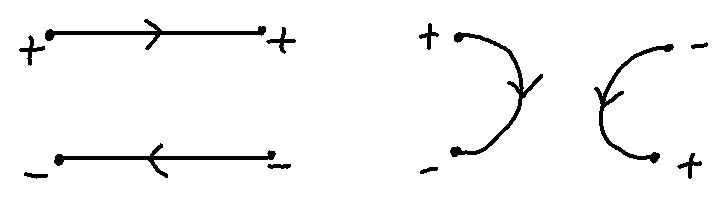
\includegraphics[width=7cm]{images/Lecture 12/generators.png} \]
    
    and the relation 
    
    \[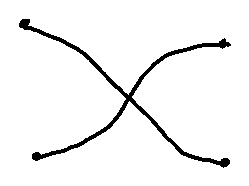
\includegraphics[width=3cm]{images/Lecture 12/relations.png} \]   
\end{lem}
\begin{proof}
    We need to show that there is a way of gluing our generators and the braiding relation to get the other 4 manifolds of \ref{class1dBord}.
    
    \begin{enumerate}
        \item   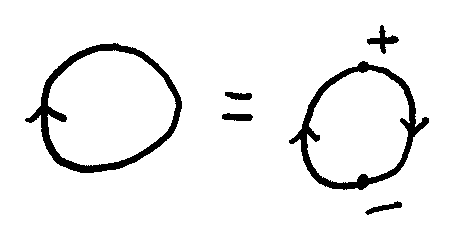
\includegraphics[width=3cm]{images/Lecture 12/circle1.png} 
        \item 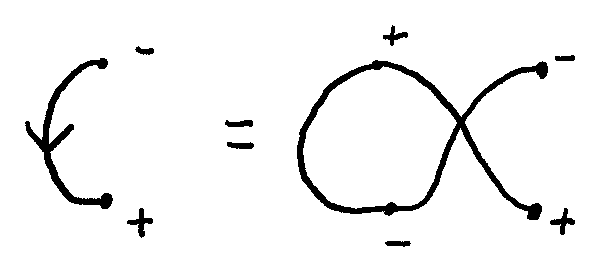
\includegraphics[width=3cm]{images/Lecture 12/coevaluationbraiding.png} 
        \item  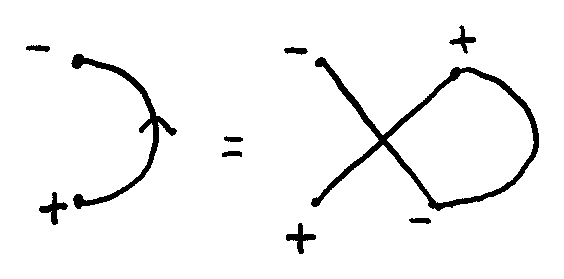
\includegraphics[width=3cm]{images/Lecture 12/evaluationbraiding.png} 
        \item 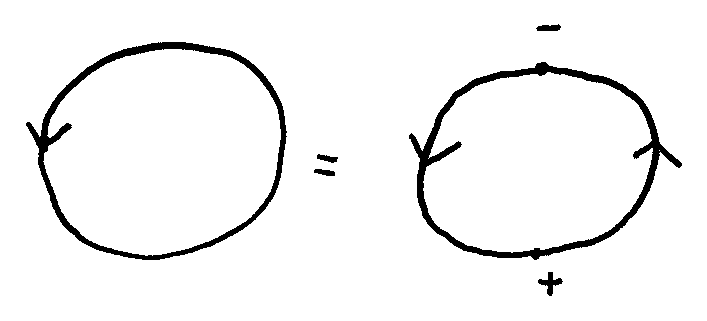
\includegraphics[width=3cm]{images/Lecture 12/circle2.png} 
    \end{enumerate}
\end{proof}
\begin{proof}[Proof of the classification of 1-TFTs]\label{abstractClass1TFT}
The moral of the latter lemma is that identity morphisms of $\bullet_{+}$ and $\bullet_{-}$, coevaluation and evaluation
    maps
    $coev_{\bullet_{+}}$ and $ev_{\bullet_{+}}$,
    and the braiding are enough to generate all the 1-dimensional bordisms.
    Thus, to determine what a TFT does, 
    we need to only determine what it does on these morphisms, i.e. 1-dimensional bordisms. In the previous lemma 
    on some properties of symmetric monoidal functors, we proved that identity morphisms are sent
    to identity morphisms,
    the co/evaluation maps are sent to co/evaluation maps and components of the braiding are sent to
    components of the braiding. Moreover, in that lemma we also proved that dual objects are sent to dual objects and
    $\bullet_{+}$ is a dual object, so for an arbitrary symmetric monoidal category $\cat$, a 1-TFT sends it to a dual object.
    From a dual object $X$ one can infer the co/evaluation maps and its dual. The braiding of a symmetric monoidal
     category is already given. 
    So we can conclude that a one dimensional TFT is fully determined by where $\bullet_{+}$ is sent to.
\end{proof}

This proof mainly relies on abstract nonsense. So we now provide an alternative proof.
 
\begin{proof}\label{GeneratorsClass1TFT}
Also this proof relies on the fact that since the functor
    is \emph{symmetric} monoidal one can just check what the TFT does only for 5 of all the possible 
    connected 1-dimensional bordisms (\ref{class1dBord}), not considering what happens for the other 3 ones with the
    reversed orientations without loss of generality because $\Bord_{1,0}$ is symmetric monoidal.
    
    First we need to determine where $\bullet_+,\bullet_-\in\Bord_{1,0}$ are sent. Since they are duals of one another,
    they are dualizable objects and thus they are sent to $X,X^{\vee}\in\cat^{\operatorname{fd}}$,
    e.g. finite dimensional vector spaces in the case of $\Vect_{k}$. An arbitrary objects of $M\in\Bord_{1,0}$
    is a finite disjoint union of $\bullet_+,\bullet_-$, i.e. 
    $$M=(\amalg_{I}\bullet_+)\amalg(\amalg_{J}\bullet_-)$$
    where $I,J\subseteq\N$. Thanks to the symmetric monoidal functoriality of $\Zf$ we have that 
    $$\Zf(M)=(\bigotimes_{I}X)\otimes(\bigotimes_{J}X^\vee)$$
    Now we need to understand where the 5 possible 1-bordisms are sent.
    \begin{enumerate}
        \item $\Zf(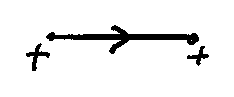
\includegraphics[scale=0.18]{images/Classification 1TFT/identityplus.png})=id_{X}$
        \item$\Zf(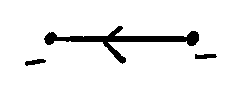
\includegraphics[scale=0.18]{images/Classification 1TFT/identityminus.png})=id_{X^\vee}$
        \item $\Zf(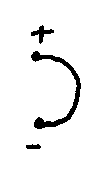
\includegraphics[scale=0.17]{images/Classification 1TFT/evaluation.png})=ev_{X}$, hence $X\amalg X^\vee\xrightarrow{ev_{X}} \unit_{\cat}$ and more precisely for $v\in X\in\Vect_{k}$: $ev_{X}:(X,\lambda)\mapsto \lambda(v)$
        \item $\Zf(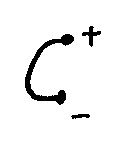
\includegraphics[scale=0.15]{images/Classification 1TFT/coevaluation.png})=coev_{X}$, hence $\unit_{\cat}\xrightarrow{coev_{X}}X\otimes X^\vee$ and more precisely for $\lambda\in k\in\Vect_{k}$, via the canonical isomorphism $X\otimes X^\vee\cong\operatorname{End}(X)$, $coev_X$ corresponds to taking the trace
        \item $\Zf(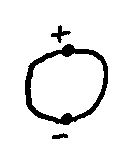
\includegraphics[scale=0.15]{images/Classification 1TFT/circle.png})=coev_X \circ ev_{X}$, hence $\unit_{\cat}\xrightarrow{coev_X \circ ev_{X}}\unit_{\cat}$, and, following the cases for $\Vect_{k}$ treated in the previous two points, to taking the trace of the identity matrix, i.e. the dimension of $X$
    \end{enumerate}
    
    The moral of the story is that a TFT is uniquely
    determined, up to isomorphism, once one knows $X\in\cat^{\operatorname{fd}}$ since then one knows 
    \begin{itemize}
        \item what $X^\vee$ is, what finite sequences of tensored $X$ and $X^\vee$ are, which will
        be sent to finite
        disjoint unions of $\bullet_{+}$ and $\bullet_-$ (aka all the objects of $\Bord_{1,0}$);
        \item what $id_X$ and $id_{X^\vee}$ are
        \item what $ev_X$ and $coev_X$ are and hence also $coev_X\circ ev_X$
    \end{itemize}
    
\end{proof}
\begin{rem}
    This proof considers 5 possible
    bordisms and not all 8, thereby excluding some possible orientations. However, Lurie's
    argument is without loss of
    generality because it implicitly relies 
    on the \emph{symmetric} monoidality of $\Bord_{1,0}$ since, for instance, one can get
    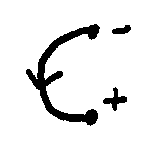
\includegraphics[width=0.7cm]{images/Lecture 12/coevminusplus.png}  by composing
    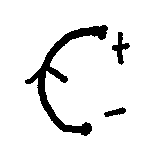
\includegraphics[width=0.7cm]{images/Lecture 12/coevplusminus.png} with a
    braiding. 
\end{rem}

We stated that these two proofs by generators and relations 
 prove the equivalence of categories in the classification of 1-TFTs. However, it might seem mysterious why this is the
  case. We now prove that the evaluation on a point is actually an equivalence of categories, a fully faithful essentially
  surjective functor by the fundamental theorem of category theory \ref{fundamentalequivalence}.

\begin{proof}
This is from \cite[Theorem 16.10]{FreedBordism}.
    
    We need to prove three things to demonstrate that $\mathcal{E}V_{\bullet_{+}}$ is an equivalence: that it is full, faithful and essentially surjective:
    \begin{enumerate}
        \item Trivially, note that since $\mathcal{E}V_{\bullet_{+}}$ lands in $(\cat^{\operatorname{fd}})^{\cong}$
        for any $A\in\cat^{\operatorname{fd}})^{\cong}$ one can define a TFT such that $\Zf(\bullet_{+})=A$
        \item It is faithful: let $\Zf,\Zf'\in \TFT_{1,0}^{or}$ and $\alpha,\beta:\Zf\Rightarrow\Zf'$ be natural
         transformations between them and hence isomorphisms (see \ref{TFTsareGRPDS}). Suppose that
          $\mathcal{E}V_{\bullet_{+}}(\alpha)=\mathcal{E}V(\beta)$, i.e. $\alpha^{1}_{\bullet_+}=\alpha^{2}_{\bullet_+}$ since $\mathcal{E}V_{\bullet_{+}}$ evaluates on the point.
        Recall that $\bullet_-=\bullet_+^\vee$. We have that for any natural isomorphism
         $\eta$ it holds that $\eta{\bullet_+^\vee}=(\eta{\bullet_+})^\vee$ because of functoriality and
          $\eta_{\bullet_-}=(\eta{\bullet_+}^\vee)^{-1}$ 
          because of \ref{DualizableMeansInvertibleNatTrans}. 
          From this it follows that
           $\alpha_{\bullet_-}=(\alpha_{\bullet_+}^\vee)^{-1}=(\beta{\bullet_+}^\vee)^{-1}=\beta_{\bullet_-}$. 
           With a specular proof we can prove that $\alpha_{\bullet_+}=\beta_{\bullet_+}$. 
           Since 0-dimensional compact manifolds are just finite disjoint unions of $\bullet_+$ or $\bullet_-$ and
            $\alpha$ and $\beta$ are symmetric monoidal natural transformations
           it follows that for any $X\in\Bord_{1,0}^{or}$, $\alpha_X=\beta_X$. 
           This proves that $\mathcal{E}V$ is faithful because it implies that for any two natural transformations that
            are mapped to equal morphisms in $\cat$ must be also equal in $\Fun^{\otimes}(\Bord_{1,0},\cat)$
        \item $\mathcal{E}V_{\bullet_{+}}$ is full. Given an arbitrary isomorphism $f:X\to X'$
         in $(\cat^{\operatorname{fd}})^{\cong}$ we now show that there is an isomorphism $\eta:\Zf\Rightarrow\Zf'$
         in $\Fun^{\otimes}(\Bord_{1,0},\cat)$ such that $\mathcal{E}V_{\bullet_{+}}(\eta)=\eta_{\bullet_{+}}=f$.
         So, we define $f=\eta$ and thus $(f^{\vee})^{-1}$.
          Objects in
          $(\cat^{\operatorname{fd}})^{\cong}$ are sequences of tensor products of $X$ and $X^\vee$. Hence,
          using the trick we used before we can extend any natural transformation $\eta:\bullet_{+}\to\bullet_{+}$
         to a disjoint union of such natural transfomations, via the monoidal structure on $\Bord_{1,0}$, since 
         any object $X\in\Bord_{1,0}$ is diffeomorphic to a finite disjoint union of $\bullet_{+}$ and $\bullet_-$, 
         and we know that
          $(\alpha_{\bullet_{+}}^{\vee})^{-1}$. This is  independent of the choice of the
           diffeomorphism between 
         $X$ and disjoint unions of $\bullet_{+}$ and $\bullet_-$ thanks to the coherence of the chosen map $\eta_{X}$.
         %I do not understand what th coherence of \eta_Y should be, naturality? Something to do with the monoidal structure? why does Freed switch continuously between X and Y for the object we are considering argh!!
         Moreover, the diffeomorphism is determined up to permutation also because of the coherence of $\eta_X$
         . It remains to show that $\eta_X$ is an isomorphism. $\eta_X$ can be a disjoint union of the 5 1-bordisms
         (\ref{class1dBord}) and hence, thanks to symmetric monoidality of $\eta$, we can just check these 5.
         The two identities are trivially isomorphisms.
         Then we need to check that the following diagram commutes to check for the coevaluation 
         % https://q.uiver.app/#q=WzAsMyxbMCwwLCJcXFpmKFxcYnVsbGV0Xy0pXFxvdGltZXNcXFpmKFxcYnVsbGV0XyspIl0sWzIsMCwiXFxaZicoXFxidWxsZXRfLSlcXG90aW1lc1xcWmYnKFxcYnVsbGV0XyspIl0sWzEsMSwiXFx1bml0X1xcY2F0Il0sWzAsMSwiZlxcY2lyYyAoZl57XFx2ZWV9KV57LTF9Il0sWzIsMCwiXFxaZihjb2V2X1gpIl0sWzIsMSwiXFxaZicoY29ldl9YKSIsMl1d
         \[\begin{tikzcd}[cramped]
            {\Zf(\bullet_-)\otimes\Zf(\bullet_+)} && {\Zf'(\bullet_-)\otimes\Zf'(\bullet_+)} \\
            & {\unit_\cat}
            \arrow["{f\circ (f^{\vee})^{-1}}", from=1-1, to=1-3]
            \arrow["{\Zf(coev_X)}", from=2-2, to=1-1]
            \arrow["{\Zf'(coev_X)}"', from=2-2, to=1-3]
         \end{tikzcd}\]
          The commutativity of this diagram follows from the fact that the following diagram commutes
        % https://q.uiver.app/#q=WzAsNixbMCwwLCJcXHVuaXRfXFxjYXQiXSxbMCwyLCJcXFpmJyhcXGJ1bGxldF8tKVxcb3RpbWVzXFxaZicoXFxidWxsZXRfKykiXSxbMCw0LCJcXFpmKFxcYnVsbGV0Xy0pXFxvdGltZXNcXFpmKFxcYnVsbGV0XyspXFxvdGltZXMgXFxaZicoXFxidWxsZXRfLSlcXG90aW1lc1xcWmYnKFxcYnVsbGV0XyspIl0sWzIsMCwiXFxaZihcXGJ1bGxldF8tKVxcb3RpbWVzXFxaZihcXGJ1bGxldF8rKSJdLFsyLDIsIlxcWmYoXFxidWxsZXRfLSlcXG90aW1lc1xcWmYnKFxcYnVsbGV0XyspIl0sWzIsNCwiXFxaZihcXGJ1bGxldF8tKVxcb3RpbWVzXFxaZicoXFxidWxsZXRfKylcXG90aW1lcyBcXFpmJyhcXGJ1bGxldF8tKVxcb3RpbWVzXFxaZicoXFxidWxsZXRfKykiXSxbMCwxLCJcXFpmJyhjb2V2X1gpIiwyXSxbMSwyLCJcXFpmKGNvZXZfeClcXG90aW1lcyBpZF97XFxaZicoXFxidWxsZXRfLSl9XFxvdGltZXMgaWRfe1xcWmYnKFxcYnVsbGV0XyspfSIsMV0sWzAsMywiXFxaZihjb2V2X1gpIl0sWzMsMiwiaWRfe1xcWmYoXFxidWxsZXRfLSl9XFxvdGltZXMgaWRfe1xcWmYoXFxidWxsZXRfKyl9XFxvdGltZXMgXFxaZihjb2V2X3gpIiwxXSxbMyw0LCJpZF97XFxaZihcXGJ1bGxldF97LX0pfVxcb3RpbWVzIGYiXSxbMiw1LCJpZF97XFxaZihcXGJ1bGxldF8tKX1cXG90aW1lcyBmXFxvdGltZXMgaWRfe1xcWmYnKFxcYnVsbGV0Xy0pfVxcb3RpbWVzIGlkX3tcXFpmJyhcXGJ1bGxldF8rKX0iLDJdLFs0LDUsImlkX3tcXFpmKFxcYnVsbGV0Xy0pfVxcb3RpbWVzXFxaZicoY29ldl94KVxcb3RpbWVzIGlkX3tcXFpmKFxcYnVsbGV0XyspfSIsMV1d
        \[\begin{tikzcd}[cramped]
            {\unit_\cat} && {\Zf(\bullet_-)\otimes\Zf(\bullet_+)} \\
            \\
            {\Zf'(\bullet_-)\otimes\Zf'(\bullet_+)} && {\Zf(\bullet_-)\otimes\Zf'(\bullet_+)} \\
            \\
            {\Zf(\bullet_-)\otimes\Zf(\bullet_+)\otimes \Zf'(\bullet_-)\otimes\Zf'(\bullet_+)} && {\Zf(\bullet_-)\otimes\Zf'(\bullet_+)\otimes \Zf'(\bullet_-)\otimes\Zf'(\bullet_+)}
            \arrow["{\Zf'(coev_X)}"', from=1-1, to=3-1]
            \arrow["{\Zf(coev_x)\otimes id_{\Zf'(\bullet_-)}\otimes id_{\Zf'(\bullet_+)}}"{description}, from=3-1, to=5-1]
            \arrow["{\Zf(coev_X)}", from=1-1, to=1-3]
            \arrow["{id_{\Zf(\bullet_-)}\otimes id_{\Zf(\bullet_+)}\otimes \Zf(coev_x)}"{description}, from=1-3, to=5-1]
            \arrow["{id_{\Zf(\bullet_{-})}\otimes f}", from=1-3, to=3-3]
            \arrow["{id_{\Zf(\bullet_-)}\otimes f\otimes id_{\Zf'(\bullet_-)}\otimes id_{\Zf'(\bullet_+)}}"', from=5-1, to=5-3]
            \arrow["{id_{\Zf(\bullet_-)}\otimes\Zf'(coev_x)\otimes id_{\Zf(\bullet_+)}}"{description}, from=3-3, to=5-3]
        \end{tikzcd}\]
    \end{enumerate}
    The argument for the evaluation of $X$ is specular. From there also the map for the circle follows since 
    the circle is just a composition of evaluation and a coevaluation with a braiding in between. Note that
    the commutativity of the circle means that $\Zf(S^1)=\Zf'(S^1)$.
\end{proof}


%\begin{proof}[Proof of the classification of 1-TFTs 2.0]
    
%   Set $\Zf( \bullet_{+})=X$ where $X\in\cat^{\operatorname{fd}}$ and $\Zf(\bullet_{-})=Y$ 
     %since we need to respect the symmetric monoidality of $\Zf$ and symmetric monoidal functors must send
    %dual objects in the source category to dual objects in the target category.
    %   $$\Zf(\bullet_+):=X$$ 
%   $$\Zf(\bullet_-):=Y$$
%   $$\Zf(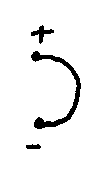
\includegraphics[scale=0.17]{images/Classification 1TFT/evaluation.png}):=ev_X$$
%   $$\Zf(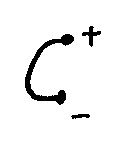
\includegraphics[scale=0.17]{images/Classification 1TFT/coevaluation.png}):=coev_X$$
%   An arbitrary compact 0-dimensional manifold
%   $M\in\Bord_{1,0}$
%   is a finite disjoint union of $\bullet_+,\bullet_-$. Thus, by a diffemorphism permuting the points 
%   $$M\cong(\amalg_{I}\bullet_+)\amalg(\amalg_{J}\bullet_-)$$
%   where $I,J\subseteq\N$. For any $M\in\Bord_{1,0}$, $\Zf$ to behave as follows, i.e. is symmetric monoidal
%%  $$\Zf(M):=(\bigotimes_{I}X)\otimes(\bigotimes_{J}Y)$$
%   By coherence of the symmetric monoidal structure, especially how the braiding and the associatior 
%%  Thanks to \ref{class1dBord}, we know that any oriented 1-dimensional bordism is diffeomorphic to a disjoint union
%   of the manifolds in \ref{class1dBord}. Since $\Zf$ is symmetric monoidal, it is sufficient to determine
%\end{proof}

The classification of 1-dimensional topological field theories is the simplest case of an
 important guiding hypothesis
 in the field of TFTs, the cobordism hypothesis, see \ref{RemarkOnCobHypo}. It is the only
  case in which so-called
 extended TFTs coincide with non-extended ones, i.e. the usual Atiyah-Segal definition as a
  simple symmetric 
 monoidal functor we are using.

%Recap: $\TFT_{1,0}^{or}(\cat) \xrightarrow{\mathscr Ev_{\bullet+}} (\cat^{\fd})^{\simeq} \hookrightarrow \cat$. The map is the following: $\Zf \mapsto \Zf(\bullet_+)$.

Now we classified 1 dimensional TFTs, we would now like to do the same for 2 dimensional TFTs.
We will find out that there is an equivalence between $\TFT_{2,1}^{or}(\cat)$ and commutative Frobenius algebra objects
in $\cat$.

\section{Classification of 2d-TFTs}
As we have done for the 1-dimensional case, we now try to classify 2-dimensional TFTs. For a more detailed proof see Kock \cite{kock_2003} or the lecture notes from Schweigert \cite{SchwHopfQuantumTFT}. 

We have already defined the following notions in arbitrary monoidal categories (see \ref{FrobAlg}, \ref{MonObj}, \ref{ComonObj}, \ref{CommFrobAlg}, \ref{CommBim}). However, we now explicitly state how the abstract formal definitions are instantiated in Vect$_k$.
\begin{defn}[Algebra over a Field]
    An algebra\footnote{Note that for us algebras are \textbf{always} associative and unital.} over a field $k$ is a monoid object (\ref{MonObj}) in $\Vect_k$. More generally a left/right $R-$algebra is a monoid object in the category of left/right $R-$modules. The latter generalization holds also for the next definitions of $k-$coalgebra, $k-$bialgebra and Frobenius $k-$algebra.
\end{defn}
\begin{defn}[Coalgebra over a Field]
    A $k-$coalgebra is a comonoid object in $\Vect_k$.
\end{defn}
\begin{defn}[Bialgebra over a Field]
    A $k-$bialgebra is a bimonoid object (see \ref{BimonObj}) in $\Vect_k$. More explicitly, it is simultaneously an $k-$algebra and a $k-$coalgebra, a monoid and a comonoid object in $\Vect_k$. 
    % the additional compatibility condition is missing /William 
    A $k-$bialgebra is commutative in $\Vect_k$, if the underlying monoid is commutative, or viceversa, if the underlying comonoid is commutative. 
\end{defn}

\begin{defn}[Frobenius $k-$Algebra]\label{Frobk-Alg}
    A Frobenius $k-$algebra is a Frobenius algebra (see \ref{FrobAlg}) in a $\Vect_k$. It is commutative if it is also a commutative $k-$algebra (and therefore a cocommutative coalgebra).
\end{defn}

These definitions are perfectly fine, if we disregard pedagogical considerations. However, they might still seem mysterious to someone not used to this abstract nonsense. For this reason, we now give three more concrete definitions of a Frobenius algebra. They are all equivalent.

% -------------------------------------------------------------
% --------------------- LECTURE 13 11/12 ----------------------
% -------------------------------------------------------------

\begin{rmnd}
    A pairing $K: W \otimes V \to k$ is non-degenerate if it is part of a data exhibiting $W$ as the dual of $V$, i.e. $\exists \gamma: k \to V \otimes W$ such that ...
\end{rmnd}

If $V,W$ finite dimensional, this is equivalent to saying that 
\begin{align}
    &K^\# : V \to W^\vee := \Hom_k(W,k), \quad v \mapsto K(- \otimes v) \\
    &K_\# : W \to V^\vee := \Hom_k(V,k), \quad w \mapsto K(w \otimes -) 
\end{align}
are isomorphisms.

\begin{exercise}
    What's the analogous reformulation of "$X \in \cat$ is dualizable"?
\end{exercise}

\begin{defn}
    A $k$-algebra is a monoid object in $\Vect_k$. More explicitly, it is a $k$-vector space $A$ together with linear maps:
    \begin{align}
        &\mu: A \otimes A \to A \\
        &\eta: k \to A
    \end{align}
    which satisfy associativity and (right and left) unitality by making the following two diagrams commute % https://q.uiver.app/#q=WzAsNSxbMCwwLCIoTVxcb3RpbWVzIE0pXFxvdGltZXMgTSJdLFsxLDAsIk1cXG90aW1lcyhNXFxvdGltZXMgTSkiXSxbMiwwLCJNXFxvdGltZXMgTSJdLFswLDEsIk1cXG90aW1lcyBNIl0sWzIsMSwiTSJdLFswLDEsIlxcYWxwaGFfe00sTSxNfSJdLFsxLDIsImlkX01cXG90aW1lc1xcbXUiXSxbMCwzLCJcXG11XFxvdGltZXMgaWRfTSIsMl0sWzMsNCwiXFxtdSIsMl0sWzIsNCwiXFxtdSJdXQ==
\[\begin{tikzcd}
    {(A\otimes A)\otimes A} & {A\otimes(A\otimes A)} & {A\otimes A} \\
    {A\otimes A} && A
    \arrow["{\alpha_{A,A,A}}", from=1-1, to=1-2]
    \arrow["{id_A\otimes\mu}", from=1-2, to=1-3]
    \arrow["{\mu\otimes id_A}"', from=1-1, to=2-1]
    \arrow["\mu"', from=2-1, to=2-3]
    \arrow["\mu", from=1-3, to=2-3]
\end{tikzcd}\]

    % https://q.uiver.app/#q=WzAsNCxbMCwwLCJcXG1hdGhiYnsxfV9cXGNhdFxcb3RpbWVzIE0iXSxbMSwwLCJNXFxvdGltZXMgTSJdLFsyLDAsIk1cXG90aW1lc1xcbWF0aGJiezF9X1xcY2F0Il0sWzEsMSwiTSJdLFswLDEsIlxcZXRhXFxvdGltZXMgaWRfTSJdLFsyLDEsImlkX01cXG90aW1lc1xcZXRhIiwyXSxbMCwzLCJcXGxhbWJkYV9NIiwyXSxbMiwzLCJcXHJob19NIl0sWzEsMywiXFxtdSIsMV1d
\[\begin{tikzcd}
    {\mathbb{1}_\cat\otimes A} & {A\otimes A} & {M\otimes\mathbb{1}_\cat} \\
    & M
    \arrow["{\eta\otimes id_A}", from=1-1, to=1-2]
    \arrow["{id_A\otimes\eta}"', from=1-3, to=1-2]
    \arrow["{\lambda_A}"', from=1-1, to=2-2]
    \arrow["{\rho_A}", from=1-3, to=2-2]
    \arrow["\mu"{description}, from=1-2, to=2-2]
\end{tikzcd}\]
    A homomorphism $\phi: A \to B$ of $k$ algebras is a linear map that preserves/commutes with $(\mu_A, \eta_A)$ and $(\mu_B, \eta_B)$, a monoid homomorphism. 
\end{defn}
\begin{defn}
    A \textit{co}algebra is a comonoid object in $\Vect_k$. More explicitly, one simply takes 
   $$ \Delta: A \to A \otimes A $$
   $$ \epsilon: A \to k $$
and reverses the arrows in the diagrams.
\end{defn}
 A homomorphisms of $k$-coalgebras accordingly preserve $(\Delta_A, \epsilon_A)$ and $(\Delta_B, \epsilon_B)$. It is a monoid homomorphism in $\Vect_k^{op}$.

\begin{ex}
    Take the vector space $A = k[x]/x^2 = k \oplus kx$ and take the map $A \to A \otimes A$ which sends $x \mapsto 1 \otimes x + x \otimes 1$ and $1 \mapsto 1 \otimes 1$ and the map $\epsilon: A \to k$ which sends 1 to 1 and $x$ to 0.
\end{ex}


\begin{defn}[First definition]
    A ($k$-) Frobenius algebra is a (finite dimensional) $k$ algebra $(A,\mu,\nu)$ together with an associative (=invariant) non-degenerate pairing $k: A \otimes A \to k$, i.e.
    \begin{equation}
        K(ab,c) = K(a, bc)
    \end{equation}
\end{defn}
The fact that the pairing is invariant actually tells us something about the algebra structure, not only the vector space structure.

\begin{ex}
    $A = \Mat_{n\times n} (k)$ with matrix multiplication, in which the pairing $K$ is simply the composition of multiplication and taking the trace, i.e. $K = \tr \circ \mu$.
    \begin{proof}
        Need to show nondegeneracy. Pick a basis of $\Mat_{n\times n} (k)$ given by $\{E_{ij}\}$ with 1 in the $j$th row and $i$th column. We then have the dual basis $\{E_{ji}\}$ and we have an isomorphism of $A$ and $A^\vee$ given by $E_{ij} \mapsto E_{ji}$. Then we can compute: $K$ is exactly the evaluation.
    \end{proof}
\end{ex}

Note that in the proof we used an isomorphism of $A$ and $A^\vee$ to get the nondegenerate invariant pairing. This leads to the following alternative definition:

\begin{defn}[Second definition]
    A ($\Phi-$) Frobenius algebra is a (finite dimensional) algebra $A$ with a left $A-$module isomorphism $\Phi: A \to A^\vee$.
\end{defn}
The left $A-$module part again gives us the compatibility with the algebra structure. 
\begin{rem}
    For the definition to make sense $A$ and $A^\vee$ should be left $A-$modules: 
    \begin{itemize}
        \item $M=A$ is an $A$ module via $A \otimes M \to M$ which sends $(a,m) \mapsto \mu(a,m)$.
        \item $M=A^\vee$ is an $A$ module via $A \otimes M \to M = A^\vee = \Hom(A,k)$ which sends $(a,\phi) \mapsto \phi(\mu(a,-))$.
    \end{itemize}
    Then a left $A-$module map should satisfy $\Phi(a \cdot m) = a \cdot \Phi(m)$.
\end{rem}
\begin{ex}
    Let's check that the map $\Phi$ in the previous example was actually a left $A-$module isomorphism. We would like
    \begin{equation}
        \Phi(A \cdot E_{ij}) = A \cdot \Phi(E_{ij})
    \end{equation}
    which is true when explicitly calculating both sides.
\end{ex}

\begin{defn}[Third definition]
    A $(\Delta, \epsilon)-$ Frobenius algebra is a finite dimensional algebra $(A,\mu,\nu)$ together with a coalgebra structure $(A,\Delta, \epsilon)$ such that the \textit{Frobenius relation} $$(\mathbb{1}_\cat\otimes\mu)\circ(\Delta\otimes\mathbb{1}_\cat)=\Delta\circ\mu=(\mu\otimes\unit_\cat)\circ(\unit_\cat itimes\Delta)$$ holds. This means that the following diagram commutes
    % https://q.uiver.app/#q=WzAsNSxbMCwxLCJBXFxvdGltZXMgQSJdLFsxLDEsIkEiXSxbMiwxLCJBXFxvdGltZXMgQSJdLFsxLDIsIkFcXG90aW1lcyBBIFxcb3RpbWVzIEEiXSxbMSwwLCJBXFxvdGltZXMgQSBcXG90aW1lcyBBIl0sWzAsMSwiXFxtdSJdLFsxLDIsIlxcRGVsdGEiXSxbMCwzLCJcXERlbHRhXFxvdGltZXMgaWRfQSIsMl0sWzMsMiwiaWRfQVxcb3RpbWVzXFxtdSIsMl0sWzAsNCwiaWRfQVxcb3RpbWVzXFxEZWx0YSJdLFs0LDIsIlxcbXVcXG90aW1lcyBpZF9BIl1d
\[\begin{tikzcd}
    & {A\otimes A \otimes A} \\
    {A\otimes A} & A & {A\otimes A} \\
    & {A\otimes A \otimes A}
    \arrow["\mu", from=2-1, to=2-2]
    \arrow["\Delta", from=2-2, to=2-3]
    \arrow["{\Delta\otimes id_A}"', from=2-1, to=3-2]
    \arrow["{id_A\otimes\mu}"', from=3-2, to=2-3]
    \arrow["{id_A\otimes\Delta}", from=2-1, to=1-2]
    \arrow["{\mu\otimes id_A}", from=1-2, to=2-3]
\end{tikzcd}\] 
\end{defn}

Note that the the only way in which we exploited the fact that we are working with vector spaces is that we had the tensor product and the unit with respect to this product. In other words, we only used the fact that $\Vect$ is a symmetric monoidal category, so the definitions work in any symmetric monoidal category\footnote{Take a detour in the subsection on monoidal categories (\ref{MonCat}), and more specifically take a look at \ref{FrobAlg}, if you want to see a definition for general monoidal categories.}. This is important to keep in mind because the target category of our 2d-TFTs might not be $\Vect_k$.

\begin{prop}
    The three definitions of Frobenius algebra are equivalent.
\end{prop}

\begin{proof}
    (1) $\iff$ (2) is an exercise.

    (3) $\implies$ (1): we set $K = \epsilon \circ \mu: A \otimes A \to k$ and $\gamma = \Delta \circ \eta$, however these are not duality data that show that $K$ is a nondegenerate pairing. 

    \noindent We can then define $\Phi: = (id_{A^\vee} \otimes K) \circ (coev_A \otimes id_A)$ which is an isomorphism with inverse $id_A \otimes ev_A) \circ (\gamma \otimes id_{A^\vee})$. Then using in addition this isomorphism one can prove that $K$ is a nondegenerate pairing.

    (1) $\implies$ (3) we can define $\Delta := \mu \circ (\gamma \otimes id_A)$ and $\epsilon := K \circ(id \otimes \mu)$.
\end{proof}

\begin{rmnd}
    $\TFT_{2,1}^{or}(\cat)$ is a groupoid (see \ref{TFTsareGRPDS}).
\end{rmnd}

%\cFrob_{\cat}^dualiz^cong right?? Since we already said that the map fctors through C^dualiz^cong /William
\begin{thm}[Classification of 2 dimensional TFTs]
    The functor 
    $$\TFT_{2,1}^{or} (\cat) \to \cFrob_{\cat}$$
    $$\Zf \mapsto \Zf(S^1)$$
    is an equivalence of groupoids\footnote{We soon prove that also the category of Frobenius algebras is a groupoid.}.
\end{thm}
The category $\cFrob_\cat$ has as objects commutative Frobenius algebras on an arbitrary symmetric monoidal category $\cat$, i.e. Frobenius algebras that are also commutative bimonoid objects (\ref{CommBim}), as morphisms it has Frobenius homomorphisms, i.e. morphisms of monoids that are also morphisms of comonoids and preserve all the structure of a Frobenius algebra. One could have also proven a statement with $\Vect_k$ as the target category and proven that $\TFT_{2,1}^{or} (\Vect_k) \simeq \cFrob_{k}$. Note that the category of commutative Frobenius algebras in an arbitrary symmetric monoidal category is indeed a groupoid: 
\begin{thm}
    The category of Frobenius algebras on an arbitrary symmetric monoidal category $\cat$ is a groupoid.
\end{thm}
%have to think about a proof for arbitrary symm mon cats, Kock just proves it for Vectk TODO
\begin{proof}
    Let $(A,\epsilon,\eta,\Delta,\mu),(A',\epsilon',\eta',\Delta',\mu')\in\cFrob_\cat$ and $\phi:A\to A'$ be a Frobenius homomorphism. Then ...
\end{proof}
Take a look at \cite{kock_2003} for a proof for Frobenius $k$-algebras, i.e. Frobenius algebras in $\Vect_k$.

\begin{proof}
    (1) We need to prove that $\Zf(S^1) =:A$ is a commutative Frobenius algebra. We get the product from the pair of pants and the coproduct from the copants. The unit and counit maps are simply given by the cup and cocup. Showing that this is actually a Frobenius algebra now just amounts to drawing the commutative diagram for a Frobenius algebra in the category of bordisms, i.e. all maps are simply bordisms.

    (2) We now want see that it's a functor. Let $\Zf, \Zf'$ be two TFTs and $\alpha: \Zf \implies \Zf'$ be a natural transformation.
    \begin{clm}
        $f = \alpha(S): A=\Zf(S^1) \to \Zf'(S^1)=B$ is a homomorphism of commutative Frobenius algebras.
    \end{clm}
    We just use naturality of $\alpha$ several times. %TODO diagram
\end{proof}


% -------------------------------------------------------------
% --------------------- LECTURE 14 13/12 ----------------------
% -------------------------------------------------------------

For functoriality we did not check that compositions of morphisms (natural transformations) are sent to compositions (of morphisms in $\cFrob$).

Now, we want to prove the converse direction: given a commutative Frobenius algebra $A$, construct an oriented 2d-TFT such that $\Zf(S^1)= A$. We want to define a TFT $\Zf$. On objects we simply set $\Zf(S^1, or_+) \mapsto A$ %TODO how to write orientation of S^1
and $\Zf(S^1, or_-) \mapsto A^\vee$. This is enough because objects in $\Bord_{2,1}^{or}$ are closed 1 dimensional manifolds and therefore diffeomorphic to a disjoint union of $S^1$s. Therefore, if $Y$ is a connected one dimensional manifold we have an orientation preserving diffeomorphism $Y \to S^1$, but in which sense is this unique? 
\begin{defn}[Diffeomorphism Group]\label{DiffeoGroup}
    Let $X\in \SmoothMfld$. $\Diff(X)$ denotes the automorphism group of $X$, i.e. the group of diffeomorphisms $X\xrightarrow{\phi}X$.
\end{defn}

Note that the diffeomorphism group can be considered a topological group (see \ref{TopologicalGroup}) if we use an apt topology, for example one can consider Diff$(X)$ a subspace of $(C^\infty(X,X),Whitney)$, where $Whitney$ denotes the \href{https://en.wikipedia.org/wiki/Whitney_topologies}{Whitney $C^\infty$ topology}, and endow it with the subspace topology.
\begin{rem}
    An isotopy (see \ref{Isotopy} for the definition) is equivalently a path in $\Diff(X)$.
\end{rem}

\begin{fct}
    Roations, SO(2) $\hookrightarrow \Diff^{or}(S^1)$ and this is a retraction.
\end{fct}
Thus, up to "wiggling", the map $Y \to S^1$ is unique. 

Upshot: for an oriented 1 manifold $Y$ we define 
\begin{equation}
    \Zf (Y) := A^{\# \pi_0(Y)} 
\end{equation}
and diffeos are sent to identities.%TODO what does this mean

Now what do we do on morphisms? 
%DRAWING
Just send everything to what we expect from the algebra and coalgebra structure! i.e. pants to multiplication, copants to comultiplication, cylinder to identity, cup to algebra unit, cocup to counit. Now, a morphism in the bordism category is a diffeomorphism class of oriented 2d bordisms and by the classification theorem we found that a 2d connected oriented manifold with boundary is diffeomorphic to a composition.
%DRAWING
A bordism then specifies where "in" and "outgoing" boundaries are. Since $\Zf$ must be functorial, given a composite as in the drawing, we must define $\Zf$ to be 
$$    \Zf(\Delta)....%TODO complete 
$$
Question: is this well defined?
%DRAWING

Going back to proof of classification, the local moves we had translate precisely to conditions of a Frobenius algebra. 
Subtlety: the following are not isomorphic as bordisms, while they are diffeomorphic as manifolds with boundary.
%DRAWING

We then need to specify what that bordism is sent to: 
\begin{equation}
    \Zf(..) : A \otimes A \xrightarrow{swap} A \otimes A
\end{equation}
So the classification of (possibly disconnected) 2d bordisms is simply a manifold with boundary as given from the classification of manifolds with boundary, composed with a permutation bordism, i.e. a bordism such as the following.
%DRAWING

Now, since $\Zf$ is functorial we simply set
\begin{equation}
    \Zf(...) %TODO complete
\end{equation}
and for well definedness consider the following drawing:
%DRAWING

but we see that this is true because the Frobenius algebra is commutative.

% -------------------------------------------------------------
% --------------------- LECTURE 15 18/12 ----------------------
% -------------------------------------------------------------

\begin{lem}
    Every (possibly non connected) 2 cobordism is a composition of 
    \begin{enumerate}
        \item a "permutation bordism". i.e. given a permutation $\sigma \in S_n$, then we get a bordism $S^{1^{1\amalg_n}} \to (S^1)^{\amalg_n}$ in which the two sides have the same orientation up to interchanging components. The bordism is simply $(S^1)^{\amalg_n}$  in which on the right we use the permutation.
        %DRAWING
        \item a disjoint union of connected 2 bordisms
        \item another permutation bordism.
    \end{enumerate}
\end{lem}

\begin{prop}
    $\Bord_{2,1}^{or}$ is the symmetric monoidal category with duals generated by (under composition and disjoint union):
    \begin{itemize}
        \item one object, $S^1$.
        \item morphisms the ones we've already mentioned: cup, pants, cocup, copants, swap (and cylinder but that's just the identity).
    \end{itemize}
    with the following relations:
    \begin{itemize}
        \item the cylinder is the identity, so composed with all the other bordisms it gives back the same boridsm
        \item sewing in disks 
        %DRAWING
        \item (co)associativity
        \item (co)commutativity
        \item Frobenius relations
    \end{itemize}
\end{prop}
In other words, $\Bord_{2,1}^{or}$  is free symmetric monoidal category with duals on one commutative Frobenius object $S^1$.

\subsection*{Usual depictions of orientations}
\label{ssub:usual_depictions_of_orientations}

%DRAWINGS

Let's now do a recap of what we've done up to now. We proved
\begin{equation}
    \TFT_{2,1}^{or}(\cat) \xrightarrow[Ev]{\simeq} \cFrob(\cat)^{\simeq}
\end{equation}
and the steps were the following:
\begin{itemize}
    \item the functor is well defined: on objects we get $Ev(\Zf) = \Zf(S^1)$ which is a commutative Frobenius algebra. On morphisms we get an isomorphism of commutative Frobenius algebras.
    \item $Ev$ is essentially surjective, actually we proved surjective.
    \item $Ev$ is fully faithful
\end{itemize}

\begin{rem}
    Last time we forgot about orientations...
    %TODO complete
\end{rem}

\section{Variants of TFTs}
We now provide an outlook to some research programs that are tightly connected to TFTs.
\begin{itemize}
    \item we could have used different tangential structures, such as
    \begin{itemize}
        \item unoriented bordisms. In this case we would need an isomorphism $A \cong A^\vee$ which should be an isomorphism of commutative Frobenius algebras.
        \item framing: not many framed closed 2 manifolds
        \item spin structure
        \item conformal structure and thereby we would have studied \emph{conformal} field theories
    \end{itemize}
    \item open-closed TFTs (Lauda-Pfeiffer, \cite{Lauda_2008}): the idea is to enlarge the bordism category to include \textit{compact} 1d manifolds (not necessarily closed) and we then also have additional morphisms.
    %DRAWINGS

    Now, what structure does the line segment have? It's still a Frobenius algebra! But it is not necessarily
     commutative.
     
      There is a more general result on the classification of such field theories by Kevin Costello
       \cite{costello2006topological}.
    
        \item extended TFTs (\cite{Freed_1994},\cite{Baez_1995},\cite{lurie2009classification},\cite{Calaque_2019}): one can extend TFTs downward, e.g. in 2-dimensional TFTs one might want to include the possibility of "composing" the line segment object with itself to get $S^1$. We would therefore modify the notion of symmetric monoidal category to be able to compose objects in $\Bord_{2,1,0}$. Thereby one gets a finer structure than a usual category, a.k.a. a $1$-category: objects, morphisms between objects and morphism between morphisms. The last ones are usually called 2-morphisms and the morphisms between objects are then called 1-morphisms. Objects, 1-morphisms and 2-morphisms are in this case 0 manifolds, 1-dimensional bordisms and 2 dimensional bordisms with corners. We then no longer have the structure of a category, but rather that of a weak 2-category, or bicategory. See \ref{strict nCat} for the definition of strict categories of any finite dimension, \ref{Bicategory} for the definition of a bicategory, and \ref{RemarkExtendedTFTs} for a more detailed outlook on extended TFTs.
    %TODO monoidal category as bicategory already done by defining delooping of a monoidal category /Andrea

    \item cohomological TFTs (\cite{Witten:1990bs}): aka families of $(n-1)$ manifolds and families of $n$ bordisms. In practice, fix a space $X$, then objects are $M$ closed $(n-1)$ manifolds together with $M \to X$ and morphisms are bordisms $\Sigma$ together with $\Sigma \to X$.

    Often we take $X=BG$ the classifying space of a group $G$ and having maps $M \to BG$ and $\Sigma \to BG$ gives us principle bundles on $M$ and $\Sigma$. This is connected to the field of \textit{gauge theory} and is sometimes called \textit{cohomological TFT}. 
%Unsure about adding these remarks on algebraic and arithmetic QFT and if it's BS, will ask Prof and please do check if BS /ANdrea
    
    \item[\extra] arithmetic field theories (\cite{Mazur1973NotesO},\cite{kim2016arithmetic},\cite{kapustin2007electricmagnetic}, \cite{Kapranov1995},\cite{RelativeBSVDUAL}): although still very conjectural, some envision poetic connections between number theory and physics via TFTs. The original intuition behind this connection is a mysterious analogy of Barry Mazur stating that number fields form correspond to some kind of 3-dimensional manifolds and primes in such number fields behave like knots embedded in these 3-dimensional manifolds. How this connects to TFTs will become clearer after the next section, where we will have gone through the connection between the Jones polynomial (a knot invariant) and 3d-Chern-Simons theory. For instance, the spectrum\footnote{Not in the sense of a modern abelian group, which we previously described \ref{Spectra Phases of Matter}! This is the spectrum of a ring.} of the commutative ring of the integers $\mathbb{Z}$ can be seen (roughly speaking\footnote{To make this more precise Mazur talks about exotic stuff like étale cohomological dimension.}) as a 3-dimensional manifold\footnote{This analogy has been
        very recently made precise by Peter Scholze via the framework of analytic stacks, which is defined
        via the language of condensed mathematics. He talked
        about this in this talk \url{https://archive.mpim-bonn.mpg.de/id/eprint/4956/}.}
        , and since the spectra prime fields can be canonically embedded in the spectra of the integers, they are analogous to knots since knots can be defined as embeddings of $S^1$ into some 3-dimensional manifold\footnote{Often it is sufficient to pick $\R^3$ as the manifold we embed in and it is what we will do in the next section. However, taking arbitrary 3 manifolds does also make sense and in some cases, like this one, it is what one desires.}. Mazur came up with this analogy in \cite{Mazur1973NotesO}, see this \href{https://mathoverflow.net/questions/50879/what-is-the-knot-associated-to-a-prime/50995#50995}{mathoverflow comment by Lieven Lebruyn}
     and the \href{https://ncatlab.org/nlab/show/Spec%28Z%29#As3dSpaceContainingKnots}{nLab entry on
         Spec($\Z$)} for accessible introductions to this specific correspondence. Some (\cite{kim2016arithmetic}, \href{https://shifted-project.github.io/}{Clark Barwick's SHIFTED project} and \href{https://www.youtube.com/watch?v=WXqmXKLtJrs}{this talk of his on his efforts towards geometric foundations for arithmetic field theories}) are trying to define arithmetic quantum field theories in order to apply ideas of TFTs to number theory, for example to arithmetic curves\footnote{Something from arithmetic geometry, see \cite{liu2002algebraic}}, i.e. the spectra of rings of integers in algebraic number fields. While others (\cite{Witten:1990bs},\cite{RelativeBSVDUAL}) more specifically, see a strong connection with the Langlands program. This view is summarized by the motto \emph{the Langlands program is part of the study of 4-dimensional (arithmetic, topological) quantum field theory}. For a more accessible introduction to this research program, check out these notes \cite{BenZviLanglands} by Jackson Van Dyke of a course on this topic by David Ben-Zvi.
    \item[\extra]\label{AQFT} algebraic quantum field theory (\cite{Haag:1963dh}): talking about endomorphism monoids, i.e. monoids of the form $(\Hom_\cat(X,X),\circ)$ (see \ref{Delooping Monoid}) we previously mentioned operator algebras, i.e. monoids and submonoids of the form $(\Hom_{\Top\!\Vect_{k}}(X,X),\circ)$. They are an object of interest in themselves but importantly for us algebraic quantum field theory makes extensive use of operator algebras. Algebraic quantum field theory is very roughly a way of translating the Heisenberg picture of quantum mechanics (sometimes called matrix mechanics) to quantum field theory by providing an attempt to axiomatize QFT in a mathematically rigorous way. Given some apt operators on an apt topological vector space, meaning that the topological vector space can represent a quantum state and the selected operators on it can represent observables, an AQFT provides a formal assignment of algebras of such operators to regions of spacetime according to some axioms, e.g. the \href{https://ncatlab.org/nlab/show/Haag-Kastler+axioms}{Haag Kastler Axioms}. In this way, it pins down how observables depend of spacetime while states are being fixed, as in the Heisenberg picture. Algebraic quantum field theory can be roughly considered to be a dual to topological quantum field theory since TFTs invert the direction by assigning geometric data to algebraic ones. In fact, topological quantum field theory can be seen as a way of translating the Schrödinger picture (also called wave mechanics) to quantum field theory: states are represented by objects in the target monoidal category, the functor from $\Bord$ captures the local time evolution, and thereby a TFT shows how states are
     propagated through time while the observables are held fixed, as in the Schrödinger picture (see more on this at \href{https://ncatlab.org/nlab/show/functorial+field+theory#QuantumMechanicsInSchroedingerPicture}{this section of the nLab entry on TFTs}). In quantum mechanics, the Heisenberg and the Schrödinger picture are two faces of the same medal, i.e. matrix mechanics and wave mechanics are equivalent\footnote{Interestingly from a historical point of view, Schrödinger's (and Eckhart's) famous proof from 1926 that the two approaches are equivalent is faulty, but von Neumann fortunately provided a foolproof demonstration in 1932. See \cite{MULLER199735} for more on this interesting trivia.}; however, we are far from proving that AQFT and TQFT are also two faces of the same medal. One point of contact between the two is via factorization algebras (something related to $E_n$-algebras, see \ref{EAlg} for the definition of a $E_1$-algebra), see
     \ref{FactorAlgebra} for a definition of factorization algebra and \cite{costello2023factorization} for
      a summary on factorization algebras and how they relate to TQFT and AQFT. 
    
    In conclusion, algebraic quantum field theory is not a variant of topological field theory, but an alternative attempt to put quantum field theory on mathematically rigorous footings. One can discover more on algebraic quantum field theory in \cite{halvorson2006algebraic} and \cite{fewster2019algebraic}.
    
 
    \item[\extra] supersymmetric field theory: supersymmetric field theories are field theories
     defined as a functor similarly to TFTs but instead of having usual manifolds in the source,
      they have objects called super manifolds. Stefan Stolz and Peter Teichner conjectured 
      a deep relation between elliptic cohomology and such quantum field theories (see \cite{TeichnerStolz}) 
      %TBD
\end{itemize}


% -------------------------------------------------------------
% ---------------------- LECTURE 16 8/1 -----------------------
% -------------------------------------------------------------

\section{3d TFTs} % (fold)
\label{sec:3d_tfts}

From now on the main reference will be \cite{KasselRossoTuraev97}.

For classifying TFTs in 1 and 2 dimensions the procedure we have been following is to find an algebraic category which is equivalent with such TFTs evaluated on some object.

\noindent In particular, in order to classify 1d TFTs (with target category $\Vect_k$) we established an equivalence via the evaluation functor of on a point, which turns out to be a finite dimensional vector spaces; while for 2d TFTs the evaluation is done on the circle $S^1$ giving us commutative Frobenius $k$-algebras.

\noindent These equivalences of categories allow us to reconstruct 1d and 2d TFTs (up to some reasonable form of equivalence) from this purely algebraic data. One can ask themselves if a classification of this kind is possible also for higher dimension, such as 3d TFTs.

\noindent First, 3d-TFTs can be constructed from algebraic data, although a bit more sophisticated than what we got in lower dimensions, we will find out that every \textit{modular tensor category} gives a 3d TFT\footnote{So-called once-extended 3d TFTs, i.e. TFTs of the sort $\Bord_{3,2,1}\xrightarrow{\Zf}\cat$, can be classified by modular tensor categories. As we previously sketched, once-extended 2d TFTs have $\Bord_{2,1,0}$ as source and $\Bord_{2,1,0}$ is a symmetric monoidal bicategory (see \ref{SymmMonBicategory} and \ref{RemarkExtendedTFTs}
    ). Also $\Bord_{3,2,1}$ is a symmetric monoidal bicategory with disjoint unions of $S^1$ as objects. In short, there is an equivalence between once-extended 3d-TFTs evaluated on the circle $S^1$ and modular tensor categories (see \cite{JordanTFTs} for more). This is a very difficult result, the details of which are not fully available yet, despite being expected/``known'' for a decade}. 

\noindent This results can be summarized diagramatically as follows
% https://q.uiver.app/#q=WzAsNixbMCwwLCJcXG9wZXJhdG9ybmFtZXtGaW5WZWN0fVxcbmkgWCJdLFswLDEsIlxcb3BlcmF0b3JuYW1le0NvbW1Gcm9ifVxcbmkgQSJdLFswLDIsIlxcb3BlcmF0b3JuYW1le01vZFRlbnNvcn1cXG5pXFxjYXQiXSxbMiwwLCJcXFpmXFxpblxcb3BlcmF0b3JuYW1lezEtVEZUfSJdLFsyLDEsIlxcWmZcXGluXFxvcGVyYXRvcm5hbWV7Mi1URlR9Il0sWzIsMiwiXFxaZlxcaW5cXG9wZXJhdG9ybmFtZXsxLVRGVH0iXSxbMCwzLCJcXHRleHR7XFx0aW55e3VuaXF1ZWx5IGRldGVybWluZXN9fSIsMCx7InN0eWxlIjp7ImJvZHkiOnsibmFtZSI6InNxdWlnZ2x5In19fV0sWzEsNCwiXFx0ZXh0e1xcdGlueXt1bmlxdWVseSBkZXRlcm1pbmVzfX0iLDAseyJzdHlsZSI6eyJib2R5Ijp7Im5hbWUiOiJzcXVpZ2dseSJ9fX1dLFsyLDUsIlxcdGV4dHtcXHRpbnl7dW5pcXVlbHkgZGV0ZXJtaW5lc319IiwwLHsic3R5bGUiOnsiYm9keSI6eyJuYW1lIjoic3F1aWdnbHkifX19XV0=
\[\begin{tikzcd}[cramped]
    {\operatorname{FinVect}\ni X} && {\Zf\in\operatorname{1-TFT}} \\
    {\operatorname{CommFrob}\ni A} && {\Zf\in\operatorname{2-TFT}} \\
    {\operatorname{ModTensor}\ni\cat} && {\Zf\in\operatorname{3-TFT}}
    \arrow["{\text{\tiny{uniquely determines}}}", squiggly, from=1-1, to=1-3]
    \arrow["{\text{\tiny{uniquely determines}}}", squiggly, from=2-1, to=2-3]
    \arrow["{\text{\tiny{uniquely determines}}}", squiggly, from=3-1, to=3-3]
\end{tikzcd}\]

\vspace{0,3cm}

Here $\operatorname{ModTensor}$ is the category of \textit{modular tensor categories}, which we will not fully
 define; rather, we give some ingredients below but you can think of them as some sort of categorified commutative Frobenius
  algebra.

\noindent The main objective of this section is to sketch how this assignment could work and what is the relation between the 3d TFT evaluated at a particular example of a modular tensor category (which is related to 3d Chern-Simons field theory) and the Jones polynomial- a knot invariant.

\noindent We beging with a somewhat strange thing:
%A modular tensor category is a tensor category with extra properties. We start with defining tensor categories.
%\begin{defn}
% A \textit{linear category} is a $\Vect_k$-enriched\footnote{See \ref{FullEnrichedCat} for a rigorous definition of what enriched is and how that works for other categories.} category, i.e.
%\begin{itemize}
%    \item $\Hom_\cat (X,Y)$ is a vector space $\forall X,Y$.
%    \item composition is bilinear $\Hom_\cat (X,Y) \otimes \Hom_\cat (Y,Z) \mapsto \Hom_\cat (X,Z)$\,.
%    
%    \noindent A \textit{tensor category} is a monoidal linear category, that is, a linear category which is monoidal, and the monoidal product on the $\Hom$s is linear.
%\end{itemize}
%\end{defn}
% TODO this can be mooved to a more categorical part, here it's a bit useless


\subsection{The Yang-Baxter equation} 
\label{ssub:the_yang_baxter_equation}

\begin{thm}\label{thm:YB_braid}
    Let \cat be a braided strict\footnote{A braided strict monoidal category is a strict monoidal category, i.e. a monoidal category where associators and unitors are strict equalities instead of natural isomorphisms, with a braiding, i.e. a natural isomorphism $-\otimes-\cong-\otimes-\circ swap$. Note that $\Vect_k$ is not an example of strict monoidal category, while a monoid or a group thought of as categories are indeed scrict. See the section on monoidal categories for more (\ref{MonCat}).} monoidal category. Then, for $U,V,W \in \cat$ we have
    $$
        (\beta_{V,W} \otimes id_U)\circ (id_V \otimes \beta_{U,W})\circ (\beta_{U,V} \otimes id_W)= (id_W \otimes \beta_{U,V}) \circ (\beta_{U,W} \otimes id_V) \circ (id_U \otimes \beta_{V,W})
    $$
    which we can visualize draw with the following ``string diagram'':
% https://q.uiver.app/#q=WzAsMjUsWzAsMCwiVSJdLFswLDEsIlYiXSxbMCwyLCJXIl0sWzIsMCwiViJdLFsyLDEsIlUiXSxbMiwyLCJXIl0sWzQsMCwiViJdLFs0LDEsIlciXSxbNCwyLCJVIl0sWzYsMCwiVyJdLFs2LDEsIlYiXSxbNiwyLCJVIl0sWzMsMywiPSJdLFswLDQsIlUiXSxbMiw0LCJVIl0sWzQsNSwiVSJdLFs2LDYsIlUiXSxbMCw1LCJWIl0sWzAsNiwiVyJdLFsyLDUsIlciXSxbMiw2LCJWIl0sWzQsNiwiViJdLFs0LDQsIlciXSxbNiw0LCJXIl0sWzYsNSwiViJdLFsxLDMsIlxccGhhbnRvbXtEfSAiLDEseyJzdHlsZSI6eyJoZWFkIjp7Im5hbWUiOiJub25lIn19fV0sWzIsNSwiaWRfe1d9IiwwLHsic3R5bGUiOnsiaGVhZCI6eyJuYW1lIjoibm9uZSJ9fX1dLFszLDYsImlkX1YiLDAseyJzdHlsZSI6eyJoZWFkIjp7Im5hbWUiOiJub25lIn19fV0sWzUsNywiXFxwaGFudG9te0R9IiwxLHsic3R5bGUiOnsiaGVhZCI6eyJuYW1lIjoibm9uZSJ9fX1dLFs3LDksIlxccGhhbnRvbXtEfSIsMSx7InN0eWxlIjp7ImhlYWQiOnsibmFtZSI6Im5vbmUifX19XSxbNiwxMCwiXFxiZXRhX3tWLFd9IiwwLHsibGFiZWxfcG9zaXRpb24iOjMwLCJzdHlsZSI6eyJoZWFkIjp7Im5hbWUiOiJub25lIn19fV0sWzgsMTEsImlkX1UiLDAseyJzdHlsZSI6eyJoZWFkIjp7Im5hbWUiOiJub25lIn19fV0sWzAsNCwiXFxiZXRhX3tVLFZ9IiwwLHsibGFiZWxfcG9zaXRpb24iOjMwLCJzdHlsZSI6eyJoZWFkIjp7Im5hbWUiOiJub25lIn19fV0sWzQsOCwiXFxiZXRhX3tVLFd9IiwwLHsibGFiZWxfcG9zaXRpb24iOjMwLCJzdHlsZSI6eyJoZWFkIjp7Im5hbWUiOiJub25lIn19fV0sWzEzLDE0LCIiLDAseyJzdHlsZSI6eyJoZWFkIjp7Im5hbWUiOiJub25lIn19fV0sWzE4LDE5LCJcXHBoYW50b217RH0iLDEseyJzdHlsZSI6eyJoZWFkIjp7Im5hbWUiOiJub25lIn19fV0sWzE3LDIwLCIiLDEseyJzdHlsZSI6eyJoZWFkIjp7Im5hbWUiOiJub25lIn19fV0sWzIwLDIxLCIiLDEseyJzdHlsZSI6eyJoZWFkIjp7Im5hbWUiOiJub25lIn19fV0sWzE5LDIyLCJcXHBoYW50b217RH0iLDEseyJzdHlsZSI6eyJoZWFkIjp7Im5hbWUiOiJub25lIn19fV0sWzIyLDIzLCIiLDEseyJzdHlsZSI6eyJoZWFkIjp7Im5hbWUiOiJub25lIn19fV0sWzIxLDI0LCJcXHBoYW50b217RH0iLDEseyJzdHlsZSI6eyJoZWFkIjp7Im5hbWUiOiJub25lIn19fV0sWzE1LDE2LCIiLDAseyJzdHlsZSI6eyJoZWFkIjp7Im5hbWUiOiJub25lIn19fV0sWzE0LDE1LCIiLDEseyJzdHlsZSI6eyJoZWFkIjp7Im5hbWUiOiJub25lIn19fV1d
\[\begin{tikzcd}[cramped]
    U && V && V && W \\
    V && U && W && V \\
    W && W && U && U \\
    &&& {=} \\
    U && U && W && W \\
    V && W && U && V \\
    W && V && V && U
    \arrow["{\phantom{D} }"{description}, no head, from=2-1, to=1-3]
    \arrow["{id_{W}}", no head, from=3-1, to=3-3]
    \arrow["{id_V}", no head, from=1-3, to=1-5]
    \arrow["{\phantom{D}}"{description}, no head, from=3-3, to=2-5]
    \arrow["{\phantom{D}}"{description}, no head, from=2-5, to=1-7]
    \arrow["{\beta_{V,W}}"{pos=0.3}, no head, from=1-5, to=2-7]
    \arrow["{id_U}", no head, from=3-5, to=3-7]
    \arrow["{\beta_{U,V}}"{pos=0.3}, no head, from=1-1, to=2-3]
    \arrow["{\beta_{U,W}}"{pos=0.3}, no head, from=2-3, to=3-5]
    \arrow[no head, from=5-1, to=5-3]
    \arrow["{\phantom{D}}"{description}, no head, from=7-1, to=6-3]
    \arrow[no head, from=6-1, to=7-3]
    \arrow[no head, from=7-3, to=7-5]
    \arrow["{\phantom{D}}"{description}, no head, from=6-3, to=5-5]
    \arrow[no head, from=5-5, to=5-7]
    \arrow["{\phantom{D}}"{description}, no head, from=7-5, to=6-7]
    \arrow[no head, from=6-5, to=7-7]
    \arrow[no head, from=5-3, to=6-5]
\end{tikzcd}\]
    where a horizontal line is the identity and a crossing is the braiding $\beta$. In the drawing we simply "moved the middle string from above to below" and this is called a \textit{Reidemeister III move} in knot theory.
\end{thm}

\noindent Note: we are used to symmetric monoidal categories and thus categories where which morphism ``goes over'' another is not relevant. For a braided monoidal category this is -in general- NOT the case, so in the diagrams above which morphism goes above and what below is important information.

\begin{proof}
    Recall that $\beta$ is a \textit{natural} isomorphism, so for $U \xrightarrow{id} U$, $V \otimes W \xrightarrow{\beta_{V,W}}W \otimes V$ we apply the naturality of $\beta_{U,-}$ and get the following diagram:
    % https://q.uiver.app/#q=WzAsNCxbMCwwLCJVXFxvdGltZXMoVlxcb3RpbWVzIFcpIl0sWzAsMSwiVVxcb3RpbWVzKFdcXG90aW1lcyBWKSJdLFsyLDEsIihXXFxvdGltZXMgVilcXG90aW1lcyBVIl0sWzIsMCwiKFZcXG90aW1lcyBXKVxcb3RpbWVzIFUiXSxbMCwxLCJpZF97VX1cXG90aW1lc1xcYmV0YV97VixXfSIsMl0sWzEsMiwiXFxiZXRhX3tVLFdcXG90aW1lcyBWfSJdLFswLDMsIlxcYmV0YV97VSxWXFxvdGltZXMgV30iLDJdLFszLDIsIlxcYmV0YV97VixXfVxcb3RpbWVzIGlkX1ciXV0=
\[\begin{tikzcd}[cramped]
    {U\otimes(V\otimes W)} && {(V\otimes W)\otimes U} \\
    {U\otimes(W\otimes V)} && {(W\otimes V)\otimes U}
    \arrow["{id_{U}\otimes\beta_{V,W}}"', from=1-1, to=2-1]
    \arrow["{\beta_{U,W\otimes V}}", from=2-1, to=2-3]
    \arrow["{\beta_{U,V\otimes W}}"', from=1-1, to=1-3]
    \arrow["{\beta_{V,W}\otimes id_W}", from=1-3, to=2-3]
\end{tikzcd}\]
    We may visualize the commutativity also via string diagrams:    
    \[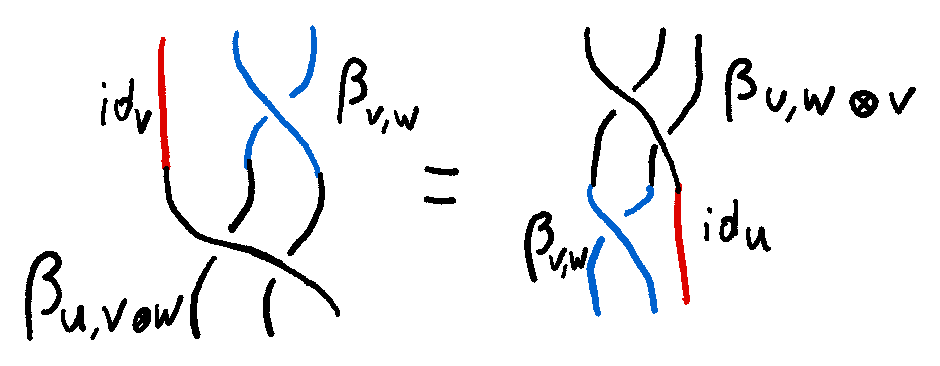
\includegraphics[width=6cm]{images/Lecture 16/stringdiagrams1.png}\]
    we get exactly two specular drawings! However, algebraically, the proof is not finished. Coming from compatibility diagrams of a braided monoida category, we have
    \begin{equation}
        (id_Y \otimes \beta_{X,Z}) \circ (\beta_{X,Y} \otimes id_Z) = \beta_{X,Y\otimes Z}
    \end{equation}
    which inserted for $\beta_{U, V \otimes W}$ and $\beta_{W \otimes V, U}$ gives the result.
\end{proof}

\noindent Now, what happens if we take $U=V=W$? Let $\beta:=\beta_{V,V}$,we now get
\begin{equation}
    (\beta \otimes id)\circ (id \otimes \beta)\circ (\beta \otimes id)= (id \otimes \beta) \circ (\beta \otimes id) \circ (id \otimes \beta)
\end{equation}
which is reminiscent of the Yang-Baxter equation (YBE):
\begin{defn}[Yang-Baxter Equation and $R$-matrix]
    Let $V$ be a vector space, $c \in \Aut(V \otimes V)$. The YBE for $c$ is 
    \begin{equation}
        (c \otimes id)\circ (id \otimes c)\circ (c \otimes id)= (id \otimes c) \circ (c \otimes id) \circ (id \otimes c)
    \end{equation}
    A solution to the YBE is called $R$-matrix. In coordinates, for $v_i$ a basis of $V$, if
    \begin{equation}
        c (v_i \otimes v_j) = \sum_{k,l} c_{ij}^{kl} v_k \otimes v_l
    \end{equation}
    then the YBE is given by
    \begin{equation}
        \sum_{p,q,y} c_{ij}^{pq}c_{qk}^{yn}c_{py}^{ln}=\sum_{y,q,r}c^{qr}_{jk}c^{ly}_{iq}c^{mn}_{yr}
    \end{equation}
\end{defn}

Theorem \ref{thm:YB_braid} then tells us that, for \textit{any} $V\in\Vect$, $\beta_{V,V}$ is an $R$-matrix! % WAT ??? Vect is NOT a strict monoidal category!!!! 

\begin{ex}
    the automorphism on $V\in\Vect$: $V \otimes V \xrightarrow{swap} V \otimes V$ satisfies the YBE because
    \begin{itemize}
        \item it comes from a standard braiding $\beta$ in $\Vect$
        \item Coxeter relation in $S_3$: $$(12)(23)(12)=(23)(12)(23)$$
    \end{itemize}

     \noindent Consider then $V$ finite dimensional vector space with basis $e_1, \dots, e_n$ and $q$ an invertible scalar. Now define $c_q (e_i \otimes e_j):= q e_i \otimes e_j $ for $i=j$, $e_j \otimes e_i$ for $i<j$ and $e_j \otimes e_i + (q-q') e_i \otimes e_j$ for $i>j$. A computation then shows that this satisfies the YBE. Note that $c_1 = swap$ is a 1-parameter "deformation" of swap.
\end{ex}

But now, this all YBE business comes from representation theory!
\begin{defn}
    Let $G$ be a group, a representation of $G$ on $V$ a vector space (or $R$ module) is a group homomorphism $\rho: G \to \Aut(V)$, i.e.
    \begin{equation}
        \rho(gh) = \rho(g) \rho(h), \quad \forall g,h \in G
    \end{equation}
    And a morphism between representations $\rho_i: G \to \Aut(V_i), i=1,2$ is a linear map $\alpha: V_1 \to V_2$ such that the following diagram commutes:
    \begin{equation}\label{eq:morphism_of_reps}
        \begin{tikzcd}
            V_1 \ar[r, "\alpha"] \ar[d, "\rho_1(g)"'] & V_2 \ar[d, "\rho_2(g)"]\\
            V_1 \ar[r, "\alpha"'] & V_2 
        \end{tikzcd}
    \end{equation}
    This gives rise to the category of representations of $G$, $\Rep_G$.
\end{defn}
\begin{rem}
    The diagram \ref{eq:morphism_of_reps} looks suspiciously like a natural transformation, and it is! In particular it's exactly example \ref{Cat of representations} in \ref{ex:natural_trafos}. In other words, the category of representations is the functor category:
    \begin{equation}
        \Rep(G) = \Fun(\mathbf B G,\Vect)
    \end{equation}
\end{rem}
\begin{ex}
    Symmetries of a polygon: $G=D_n$ dihedral group and $\rho: D_n \to \Aut(\R^2)$, where $D_n \acts \R^2$ via
     reflections and rotations. For example the reflections can be represented visually for the hexagon as follows
    \[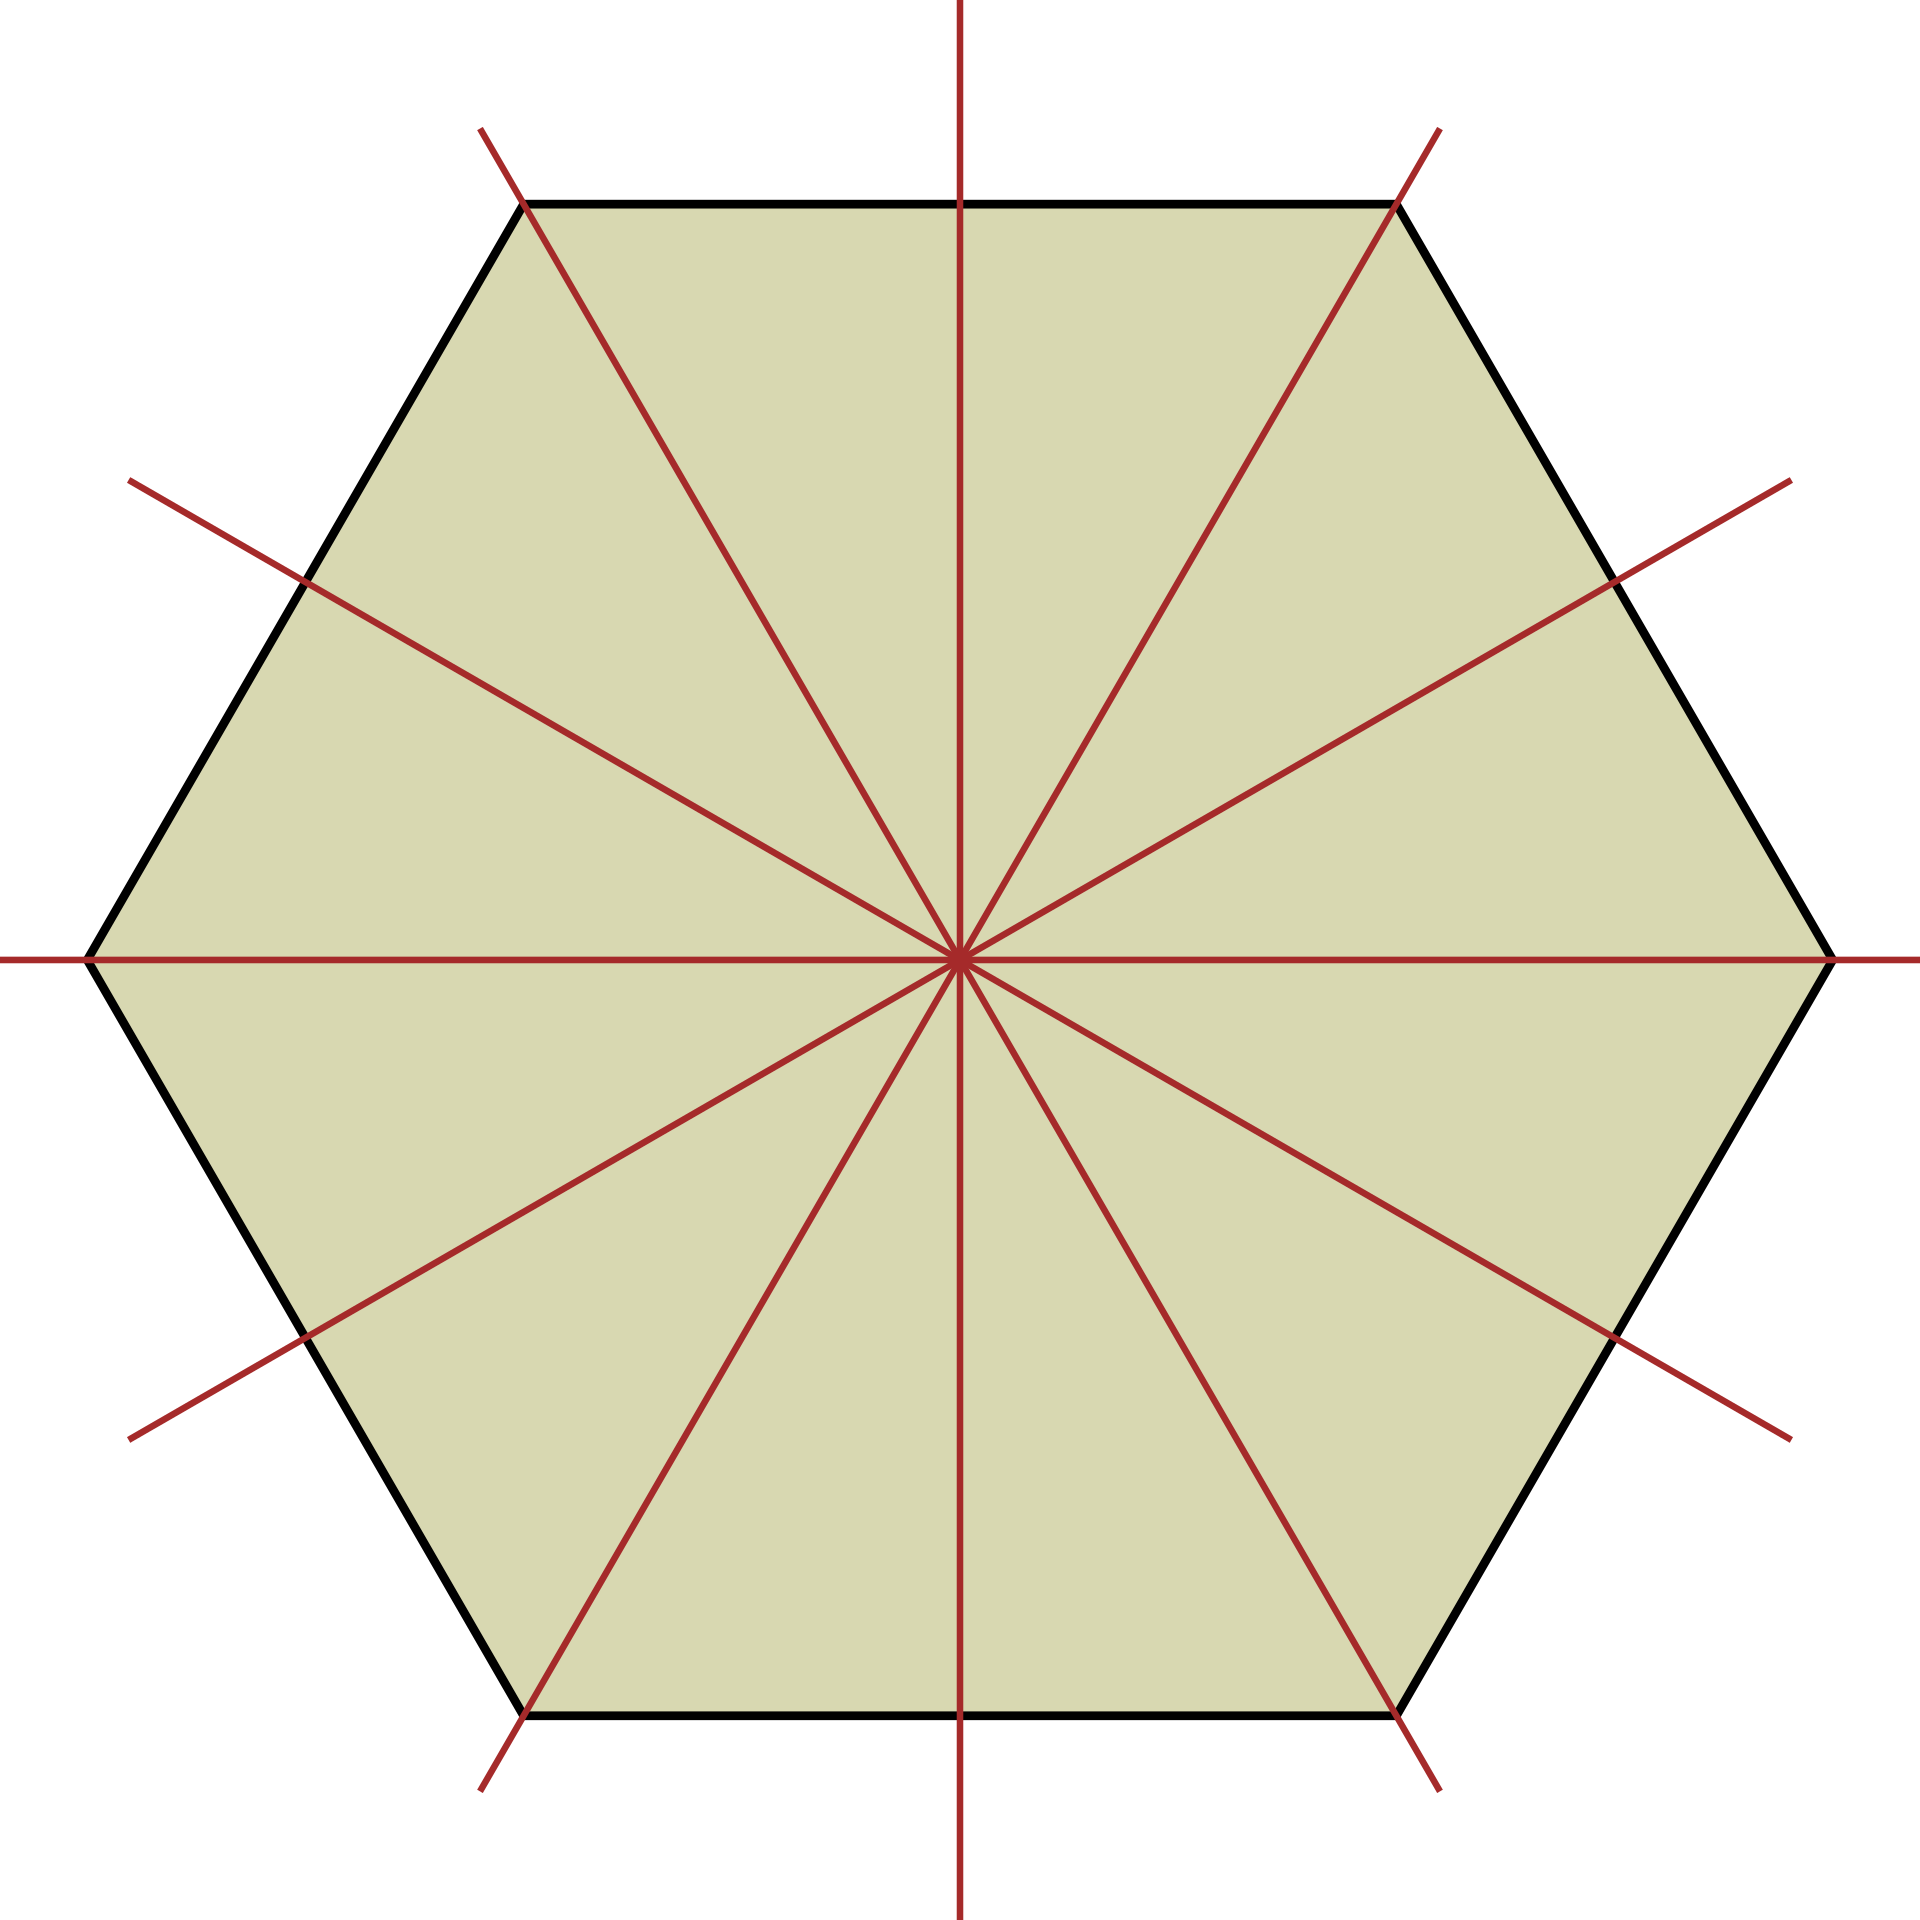
\includegraphics[width=4cm]{images/Lecture 16/Hexagonsymmetries.png}\]
\end{ex}

Solutions of YBE give representations of the braid group, which we explore in the next section.

\subsection{The braid group and the Braid category} % (fold)
\label{ssub:the_braid_group}

\begin{defn}[Braid groups]
\label{defn:braid_group}
    Let $k\geq 3$. The braid group $B_k$ with $k$ strands has $k-1$ generators $\sigma_1, \dots, \sigma_{k-1}$ and 2 relations:
    \begin{flalign}
        \label{eq:braid_relations}
        \quad
        \begin{matrix*}[l]
            1.\;\sigma_i \sigma_j  = \sigma_j \sigma_i &\text{if} \quad |i-j|>1 \\
            2.\;\sigma_i \sigma_{i+1} \sigma_i = \sigma_{i+1} \sigma_i \sigma_{i+1} &\text{if}\quad 1\leq i<k-1 \\
        \end{matrix*}&&
    \end{flalign}
    % \begin{enumerate}
    %     \item $\sigma_i \sigma_j = \sigma_j \sigma_i$ if $|i-j|>1$
    %     \item $\sigma_i \sigma_{i+1} \sigma_i = \sigma_{i+1} \sigma_i \sigma_{i+1}$ for $1\leq i<k-1$
    % \end{enumerate}
    In addition $B_2$ is the free group on one generator $\sigma$, i.e. it is isomorphic to $\Z$. For
    even lower generators $B_1 = B_0 = {e}$.
\end{defn}
\noindent The reason we call $B_k$ the braid group with $k$ strands is that we can picture the elements $\sigma_i$ in the following way:
\[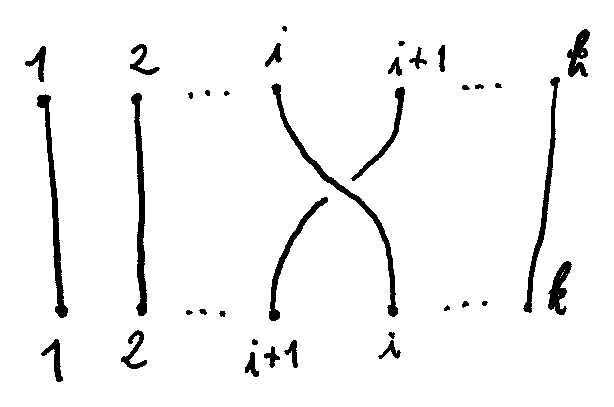
\includegraphics[width=4cm]{images/Lecture 16/BraidGroup.png}\]
which resembles a braid.
\begin{rem}
    There is a surjective homomorphism to the symmetric group
    \begin{equation}
        \begin{tikzcd}[row sep=tiny, column sep=small]
            B_k \ar[r] & S_k \\
            \sigma_k \ar[r, mapsto] & s_k
        \end{tikzcd}
    \end{equation}
    which is clear since $S_k$ has the same generators and relations with in addition $s_i^2=e$.
\end{rem}

\begin{prop}\label{prop:Rmatrix_reptheory}
    Let $c \in \Aut(V \otimes V)$ be an $R$-matrix (i.e. a solution of the YBE). Then, for any $k >0$, there is a unique homomorphism $\rho_k^c: B_k \to \Aut(V^{\otimes k})$ (i.e. a representation of $B_k$ on $V^{\otimes k}$) such that
    \begin{equation}
        \rho_k^c (\sigma_i):= c_i, \quad i=1, \dots, k-1
    \end{equation}
    with the $c_i\in \Aut(V^{\otimes k})$ is defined as: take $c$ in position $i, i+1$ and id otherwise, i.e.
    \begin{equation}
        c_i := 
        \begin{cases}
            c \otimes id_{V^{\otimes(k-2)}}, &i=1 \\
            id_{V^{\otimes(i-1)}} \otimes c \otimes id_{V^{\otimes(k-i-1)}}, & 1<i<k-1 \\
            id_{V^{\otimes(k-2)}} \otimes c, & i=k-1    
        \end{cases}
    \end{equation}
    (the second expression alone is enough is we forget about the identity when we have $id_{V^{\otimes 0}}$)
\end{prop}
% so R matrices give us representations of the Braid groups, is the converse also true?
\begin{rem}
    With this notation, YBE reads as 
    \begin{equation}
        c_1 c_2 c_1 = c_2 c_1 c_2
    \end{equation}
    since the extra identities have no relevant effect. Equivalently then the YBE can also be written as 
    \begin{equation}
        c_i c_{i+1} c_i = c_{i+1} c_i c_{i+1}
    \end{equation}
\end{rem}

\begin{proof}
    Define $\rho_k^c (\sigma_i):= c_i$ and check that the $c_i$ satisfy the relations in Definition \ref{defn:braid_group}. 

    \noindent For 1. we would like
    \begin{equation}
        c_j c_i
        = 
        c_i c_j 
    \end{equation}
    for $i > j+1$. This follows from the fact that $c_i$ and $c_j$ don't "interact":
    \begin{align*}
        &
        (id_{V^{\otimes(j-1)}} \otimes c \otimes id_{V^{\otimes(k-j-1)}})
        (id_{V^{\otimes(i-1)}} \otimes c \otimes id_{V^{\otimes(k-i-1)}}) 
        \\
        =&
        (id_{V^{\otimes(j-1)}} \otimes c \otimes id_{V^{\otimes(i-j-2)}}\otimes id_{V^{\otimes 2}} \otimes id_{V^{\otimes(k-i-1)}}) 
        (id_{V^{\otimes(i-1)}} \otimes c \otimes id_{V^{\otimes(k-i-1)}})
        \\
        =&(id_{V^{\otimes(j-1)}} \otimes c \otimes id_{V^{\otimes(i-j-2)}} \otimes c \otimes id_{V^{\otimes(k-i-1)}} )\\
        =&
        (id_{V^{\otimes(i-1)}} \otimes c \otimes id_{V^{\otimes(k-i-1)}}) 
        (id_{V^{\otimes(j-1)}} \otimes c \otimes id_{V^{\otimes(k-j-1)}})
    \end{align*}

    \noindent 2. simply follows from the remark above.
\end{proof}

% -------------------------------------------------------------
% ---------------------- LECTURE 17 10/1 ----------------------
% -------------------------------------------------------------

Now we would like to know a geometrical interpretation of the braid group: for this we need to talk about the configuration space.
%TODO check reference for names...
\begin{defn}[Unordered configuration space]
    Let $\uConf_k(\R^2) \subset (\R^2)^k$ be the subspace of $k$-tuples $(x_1, \dots, x_k)$ such that $x_i \neq x_j$ for $i\neq j$, this space is called the \textit{ordered} configuration space.
    Then we have an action $S_k \acts \uConf_k(\R^2)$. 
    The \textit{unordered} configuration space is $\Conf_k(\R^2) := \uConf_k(\R^2)/S_k$.
\end{defn}

You should thing of $\uConf_k(\R^2)$ as the collection of all possible (ordered, meaning that we give a number to each point) $k$ distincts point on the plane. $\Conf_k(\R^2)$ is the same but now we forget about the numbering.

% Distinguished configuration... %TODO complete, was this just the choice of p or what /William
\noindent We would like to talk about the fundamental group of $\Conf_k(\R^2)$ (the why will become clear in a moment), but for that we need to pick a basepoint. Let us indicate coordinates by working in \C rather than in $\R^2$. Then let $p = [(1, 2, \dots, k)] \in \C^k$, that is to say that all points are placed on the $x$-axis in steps of 1 (and the square brackets are to indicate the class under the quotient by $S_k$).
\noindent We then have a homomorphism $B_k \to \pi_1(\Conf_k(\R^2), p)$ which sends $\sigma_i \mapsto \hat \sigma_i = [f_i]$ where $f^i$ is a loop at $p$, defined in $(\R^2)^k$ by:
\begin{equation}
    f^i = (f_1^i, \dots, f_k^i): [0,1] \to (\R^2)^k \cong \C^k
\end{equation}
\begin{align}
    f^i_j(s) &= j, \quad \text{if } j \neq i, i+1 \\
    f^i_i(s) &= \frac{1}{2} (2i+1 - e^{\pi i s}) \\
    f^i_{i+1}(s) &= \frac{1}{2} (2i+1 - e^{\pi i s}) 
\end{align}
this indeed induces a loop in $\Conf_k (\R^2)$.

\noindent For it to be a homomorphism we need to check that the images of $\sigma_i$ satisfy the relations \ref{eq:braid_relations} of the $B_k$ group.
\begin{enumerate}
    \item $\hat\sigma_i \hat\sigma_j = \hat\sigma_j \hat\sigma_i$ for $|i-j|>1$
    \item $\hat\sigma_i \hat\sigma_{i+1} \hat\sigma_i = \hat\sigma_{i+1} \hat\sigma_i \hat\sigma_{i+1}$ for $1\leq i<k-1$
\end{enumerate}
For 1. one finds the same result as in the proof of Proposition \ref{prop:Rmatrix_reptheory} above, i.e. for $|i-j|>1$, $\hat\sigma_i$ and $ \hat\sigma_j$ don't "interact" with one another. Instead 2. can be checked visually.
%DRAWING

\noindent The following important result can be found in \cite{Artin1950}. 
\begin{thm}
    This homomorphism $\phi: B_k \to \pi_1 (\Conf_k(\R^2),p)$ is an isomorphism.
\end{thm}

The drawings above may give us the idea to construct a category in which morphisms are given by the paths $f$ which are morphisms between sets $k$ points. This will be the Braid category.
\noindent More in detail, given a representative $f = (f_1, \dots, f_k): [0,1] \to (\R^2)^k$ of an element in $\pi_1(\Conf_k(\R^2),p)$ we can define the following subset of $[0,1] \times \R^2$:
\begin{equation}
    L_f = \bigcup_{j=1}^k \{(s, f_j(s)): s \in [0,1]\}
\end{equation}
which is pretty much what we were drawing above, the graph of the path considered. It is therefore simply the union of disjoint line segments.
Note now that
\begin{enumerate}
    \item $\de L_f = \{0,1\} \times \{1,2, \dots, k\}$ since the path starts and ends at $p=[(1, 2, \dots, k)]$.
    \item $\forall s \in [0,1]$ we have that $L_f \cap (\{s\} \times \R^2) = k$ points.
    \item $L_f$ is a bordism from $\{1,\dots, k\}$ to itself. Where in addition we can add an orientation by "flowing" from 0 to 1.
    \item group structure gives the composition of bordisms.
    \item always have just $\bullet_1, \dots, \bullet_k$ as source/target $\implies$ can take just this object.
    \item bordism $L_f$ comes with an embedding into $[0,1] \times \R^2$. This really depends on the representative! But the bordism itself only depends on $[f] \in \pi_1(\Conf_k(\R^2))$.
    %DRAWING
\end{enumerate}

\noindent This allows us to define the following category:
\begin{defn}
    The $\Braid$ category is given by:
    \begin{itemize}
        \item objects: natural numbers $0, 1, \dots, k, \dots$, which we think of as sets of $k$ points,
        \item morphisms: 
            \begin{equation}
                 \Hom_{\Braid}(k,l) = 
                 \begin{cases}
                     \emptyset & \text{if } k \neq l \\
                     \text{isotopy classes of "braids" from $k$ to $k$} & \text{if } k = l
                 \end{cases}
                 %& \emptyset\quad \text{if } k \neq l\\
                 %& \text{isotopy classes of "braids" from $k$ to $k$}
             \end{equation} 
             By braids we mean a "permutation 1 bordism together with an embedding" $\bigcup_{\{1, \dots, k\}} [0,1] \hookrightarrow [0,1] \times \R^2$ such that 1. and 2. hold.
             %I think 1. is implied and we only need 2 /William
         \item composition is "stacking the pictures", i.e. composition of bordisms plus stacking embeddings (using $[0,1] \cup_{1=0} [0,1] \cong [0,1]$). 
         \item braided monoidal structure given pictorially by stacking $\R^2$s next to each other, in the sense that $k \otimes l = k+l$ in which the additional $l$ points are simply stacked next to the initial $k$ points. 
         %(using embedding $\R^2 \amalg \R^2 \cong [0,1]^2 \amalg [0,1]^2 \hookrightarrow \R^2 \cong [0,1]^2$).
    \end{itemize}
\end{defn}

\begin{exercise}
    One could now prove that $\Braid \simeq \coprod_{k\geq 0} B_k$, where $\coprod_{k\geq 0} B_k$ was in one of the exercise sheets. 
    %Isomorphism or equivalence of categories? /William
\end{exercise}

\subsection{Expanding the Braid category: the Tangle category} % (fold)
\label{ssub:expanding_the_braid_category_the_tangle_category}

Next step: allow more morphisms, namely all bordisms, together with suitable embeddings.
\begin{defn}
    A tangle with $k$ inputs and $l$ outputs is a 1 dimensional bordism $\Sigma$ from $k$ to $l$ points together with $\Sigma \hookrightarrow [0,1] \times \R^2$ smooth embedding, such that
    \begin{align}
        \de_{in} \Sigma &= \{(0,1), (0,2), \dots, (0,k)\}\\
        \de_{out} \Sigma &=\{(1,1), (1,2), \dots, (1,l)\}
    \end{align}
\end{defn}
%DRAWING example

\noindent We can now define the tangle category, of which $\Braid$ will be a (braided monoidal) subcategory.
\begin{defn}
    The tangle category $\Tang_1$ has:
    \begin{itemize}
        \item objects: natural numbers
        \item morphisms: 
        \begin{equation}
            \Hom_{\Tang_1}(k,l) = \{\text{isotopy classes of tangles from $k$ to $l$ points}\}
            %TODO specify somewhere what we mean by isotopy
        \end{equation}
        \item composition of underlying bordisms and stacking embeddings
        \item braided monoidal structure as before
    \end{itemize}
\end{defn}
\noindent Note that we also have $\Braid \subset \Tang_1$.

%I think we already have this def /William
\begin{defn}
    Let $(\cat, \otimes)$ be a monoidal category and $X \in \cat$. We say that $Y$ is a right dual of $X$ if there is 
    \begin{align}
        ev_X&: Y \otimes X \to 1 \\
        coev_X&: 1 \to X \otimes Y
    \end{align}
    such that the snake relations are satisfied. We then say that $X$ is a left dual of $Y$. See \ref{DefDualObj} for a complete defintition.
\end{defn}

\begin{lem}
    In $\Tang$, every object has a left and a right dual.
\end{lem}
\begin{proof}
    Same pictures as for $\Bord_1$.
\end{proof}

% -------------------------------------------------------------
% ---------------------- LECTURE 18 15/1 ----------------------
% -------------------------------------------------------------

%TODO probably already written
% \begin{defn}
%     A tangle with $k$ inputs and $l$ outputs is a one dimensional bordism $\Sigma$ from $k$ points to $l$ points together with a smooth embedding $\Sigma \hookrightarrow [0,1] \times \R^2$ such that
%     \begin{itemize}
%         \item $\de_{in} \Sigma = \{(0,1), (0,2), \dots , (0,k)\}$
%         \item $\de_{out} \Sigma = \{(1,1), (1,2), \dots , (1,l)\}$
%     \end{itemize}
%     This gives a braided monoidal category $\Tang_1 \supset \Braid$.
% \end{defn}
% DRAWING

We can now define the concept of a framing on a tangle, which is different from what we previously meant as framing.
\begin{defn}
    A framing on a tangle  is a nonvanishing normal vector field on the tangle such that at the in-boundary and at the out-boundary it "points up".
\end{defn}
\noindent This definition is made clearer through examples:
\begin{ex}
    ...
    %DRAWING
\end{ex}

Considering framed tangles leads to the \textit{framed} tangle category $\Tang_1^{fr}$.

\noindent In fact, on the line segment as a bordism between two points we have \Z many non isotopic framings corresponding to the \textit{winding number} of normal vector fields. Similarly, $S^1$ also has \Z many framings. 

\noindent We noted last time that $\Tang_1$ has left and right duals, one can check now that $\Tang_1^{fr}$ also does. We see that the framed tangle category is very similar but it has \Z many morphisms between two points, instead of just one. This idea can be generalized with the concept of a ribbon category:
\begin{defn}
    A ribbon category is a braided monoidal category \cat in which:
    \begin{enumerate}
        \item every object $X$ has a right dual $X^\vee$, thus satisfying  $$ev_X : X^\vee \otimes X \to 1$$ $$coev_X: 1 \to X \otimes X^\vee$$ which satisfies the snake relations/triangle identities (\textit{right rigid category}),
        \item there is a pivotal structure, that is a  monoidal isomorphism
        \begin{equation}
            w: id_\cat \implies ( -)^{\vee\vee}
        \end{equation}
        (these two properties are the defining ones for a \textit{pivotal category})
        \item For any object $X$, we have a "twist"
        \begin{equation}
            \vartheta_X = (id \otimes ev_{X^\vee}) \circ (\beta_{X,X} \otimes id) \circ( id_X \otimes coev_X)
        \end{equation}
        This satisfies 
        \begin{equation}
            (\vartheta_X)^\vee  = \vartheta_{X^\vee}
        \end{equation}
        %this an extra condition right? not just a fact /William
    \end{enumerate}
    Here we're using an abuse of notation, by identifying $X^{\vee \vee}$ with $X$.
%TODO diagram
\end{defn}

\begin{ex}
    In $\Tang_1^{fr}$, the $\vartheta$ is exactly the picture with the blackboard framing. It remains to check property 3, which will be an exercise.
\end{ex}

The definition of the dual of a map $f: X \to Y$ was given in \ref{DualMorph} and is given by the following composition:
$$f^\vee:Y^\vee\xrightarrow{id_{Y^\vee} \otimes coev_X}Y^\vee\otimes X \otimes X^\vee\xrightarrow{id_Y^\vee\otimes f\otimes id_{X^\vee}}Y^\vee\otimes Y\otimes X^\vee\xrightarrow{ev_Y\otimes id_{X^\vee}}X^\vee$$

%TODO maybe add explicit calculation /William

\begin{lem}
    Let \cat be a braided pivotal category. Then every object has a left dual, the twist is invertible and natural in $X$ and $\vartheta_\unit = id_\unit$ and
    \begin{equation}
        \vartheta_{X \otimes Y} = \beta_{Y,X} \circ \beta_{X,Y} \circ \vartheta_X \otimes \vartheta_Y
    \end{equation}
\end{lem}
%I don't know if this was said in class but it was in the script /William
\begin{notat}
    We denote the left dual of $X$ by $({}^\vee X, \tilde{ev_X}, \tilde{coev_x})$.
\end{notat}

\begin{ex}
\hfill
    \begin{itemize}
        \item $\Vect_k^{finite dim}$ is a ribbon category with the usual tensor product and braiding.
        \item $\Mod_R^{fpp} = R-\Mod^{fpp}$ is a ribbon category, where $fpp$ stands for finitely presented and projective and $R$ is a ring or $k$ algebra.
    \end{itemize}
    However both these examples are \textit{symmetric} monoidal
\end{ex}
\noindent We would also like some more examples which are braided but \textit{not} symmetric.

%so here we mean algebra over a ring while before was algebra over field? Or what's the difference /William
\noindent In order to do so, consider an algebra $A$, then $A-\Mod$ is a category. Now, which extra structure on $A$ guarantees that $A-\Mod^{f.d.}$ is ribbon? Section \ref{ssub:making_} below is dedicated to answering this question. As a small preview we will be dealing with:
\begin{itemize}
    \item representations of "quantum groups":
    \begin{itemize}
        \item a "deformation" of $\Rep G = \Mod U\g$, %why is this true?/William
        \item equivalently, a deformation of $U\g$ as a "Hopf algebra";
    \end{itemize}
    \item representations of a "ribbon Hopf algebra" $H$ which is a Hopf algebra with additional structure. We'll find $H-\Mod^{f.d.}$ to be a ribbon category. In particular we'll concentrate on $G=SL_2$ and we take $H = U_q (\sl_2)$ where $q$ is a root of unity.
\end{itemize}

Before that, we define a variation of the tangle category above and we'll have an interlude on knot theory.
\begin{defn}
    Let \cat be a ribbon category. $\Tang_1^{fr}(\cat)$ is the following ribbon category, in which we "decorate with objects in \cat".
    \begin{itemize}
        \item objects: finite sequences
            \begin{equation}
                (V_1, \epsilon_1), \dots, (V_k, \epsilon_k)
            \end{equation}
            where $V_i \in \cat$ and $\epsilon_i = \pm 1$. This corresponds to $k$ points in $\Tang_1^{fr, or}$ in which $\epsilon$ gives us the orientation of each point.
        \item morphisms: has underlying (isotopy classes of) framed oriented tangles + each component is labelled by $V \in \cat$ such that the source and target are labelled by $(V, \pm 1)$.
        \item Composition is stacking pictures but only if the labels match up.
    \end{itemize}
    The "correspondence" above is actually a forgetful functor $\Tang_1^{fr}(\cat) \to \Tang_1^{fr, or}$, in which $or$ means adding an orientation to the bordism.
\end{defn}

\begin{prop}
    If \cat is a ribbon category, then there is a unique braided monoidal functor $F : \Tang_1^{fr} (\cat) \to \cat$ such that
    \begin{itemize}
        \item $F(V, +1) = V$ and $F(V, -1) = V^\vee$
        \item $\forall V, W \in \cat$ we have:
        %DRAWING
    \end{itemize}
\end{prop}

Finally, what does all this have to do with 3d TFTs? 
% https://q.uiver.app/#q=WzAsNCxbMCwwLCJcXFRhbmdee1xcZnJ9X3sxfShcXGNhdCkiXSxbMCwyLCJcXEJvcmRfezN9Il0sWzEsMCwiXFxjYXQiXSxbMiwwLCJcXFZlY3QiXSxbMCwxLCJcXG9wZXJhdG9ybmFtZXtzdXJnZXJ5IH0iLDIseyJzdHlsZSI6eyJ0YWlsIjp7Im5hbWUiOiJhcnJvd2hlYWQifSwiYm9keSI6eyJuYW1lIjoic3F1aWdnbHkifX19XSxbMCwyXSxbMiwzLCJmb3JnZXQiXSxbMSwzXV0=
\[\begin{tikzcd}[cramped]
    {\Tang^{\fr}_{1}(\cat)} & \cat & \Vect \\
    \\
    {\Bord_{3}}
    \arrow["{\operatorname{surgery }}"', squiggly, tail reversed, from=1-1, to=3-1]
    \arrow[from=1-1, to=1-2]
    \arrow["forget", from=1-2, to=1-3]
    \arrow[from=3-1, to=1-3]
\end{tikzcd}\]
We will use:
\begin{itemize}
    \item every $3$-manifold arises from framed 1-tangles via \textit{surgery},
    \item two tangles giving the same 3 manifold can be related by \textit{Kirby moves},
    \item $F_\cat$ is invariant under Kirby moves if \cat is a \textit{modular} tensor category.
\end{itemize}

% -------------------------------------------------------------
% ---------------------- LECTURE 19 22/1 ----------------------
% -------------------------------------------------------------

\subsection{Interlude on knots, links and the Jones polynomial} % (fold)
\label{sub:interlude_on_knots_links_and_the_kones_polynomial}

\begin{ex}

    Examples of knots are the following:
    \begin{itemize}
        \item the \textit{unknot} \[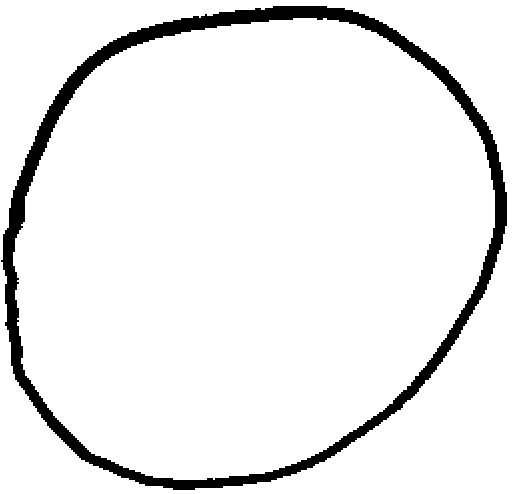
\includegraphics[width=2.5cm]{images/Lecture 19/unknot.png}\]
        \item the \textit{trefoil} \[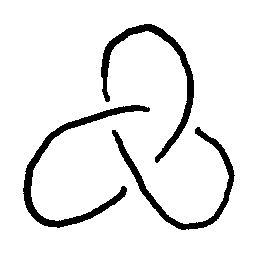
\includegraphics[width=2.5cm]{images/Lecture 19/trefoil.png}\]
        \item the \textit{figure 8 knot} \[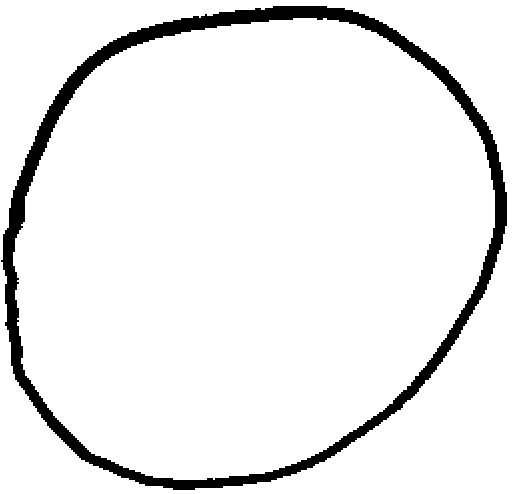
\includegraphics[width=2.5cm]{images/Lecture 19/unknot.png}\]
        
    \end{itemize}
    and of links:
    \begin{itemize}
        \item the \emph{Hopf link}  \[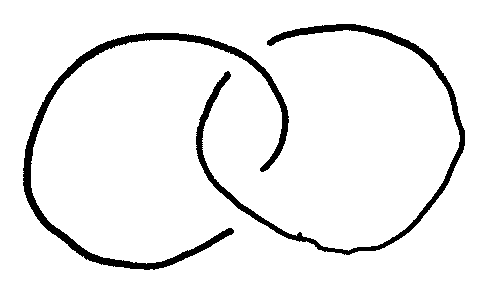
\includegraphics[width=2.5cm]{images/Lecture 19/Hopflink.png}\]
        \item the \emph{Borromean rings}  \[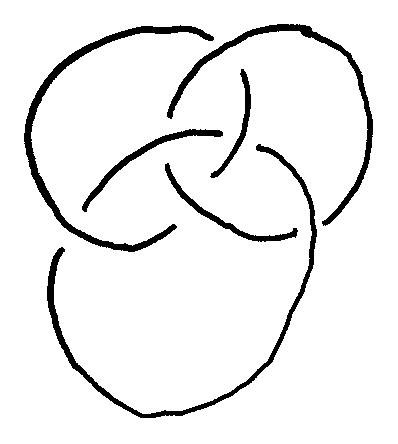
\includegraphics[width=2.5cm]{images/Lecture 19/Borromeanrings.png}\]
    \end{itemize}
\end{ex}
\begin{rem}[Knots and links as symbols \extra]
The Borromean rings are called 'Borromean' because they appear on the coat of arms of a noble family from Northern
Italy named 'Borromeo'. However, this is not the only instance of such link in history. They often appear elswhere
 with fascinating symbolism. For instance,
 they also symbolized the trinity
\[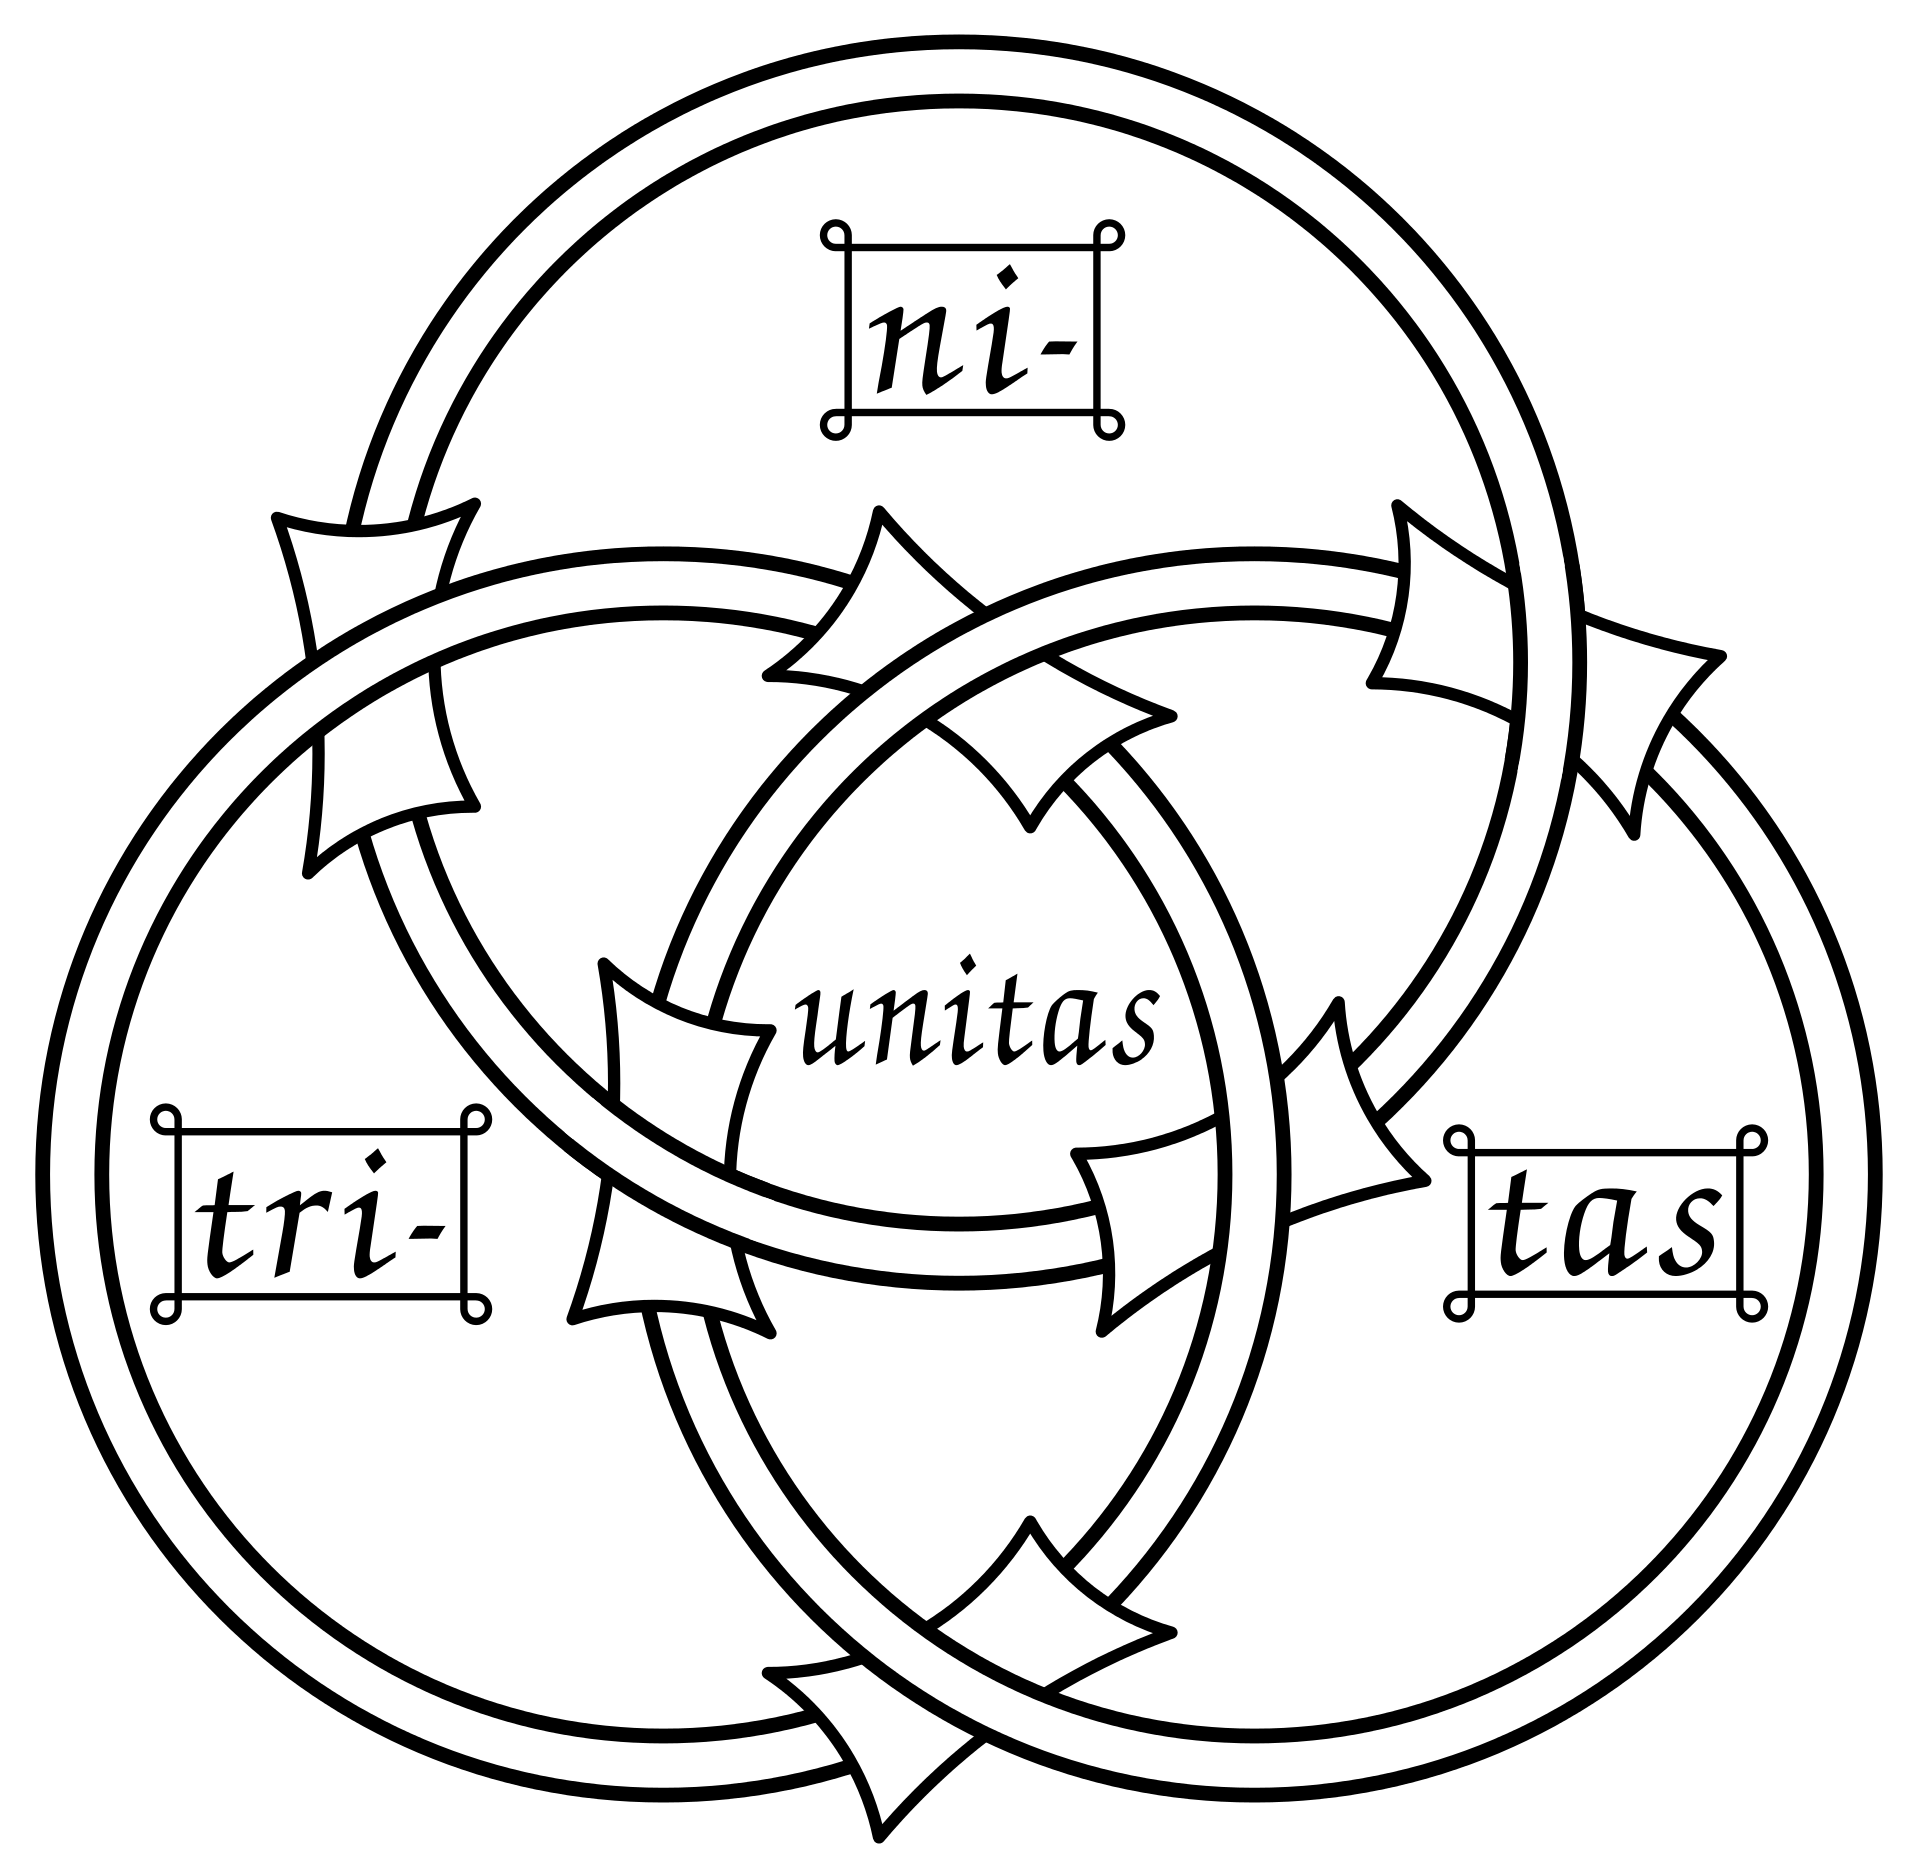
\includegraphics[width=2.5cm]{images/Lecture 19/BorromeanRings-Trinity.png}\]
Interlocked triangles, which we now refer
to as 'valknut', often appear in areas inhabited by Germanic peoples. Sometimes the valknut symbolizes the pagan
 God Odin. 
Some of these valknuts are topologically equivalent to the Borromean rings, such version is called the tricursal
 valknut. 
 Here is an example of a tricursal valknut on an 
ornate slab of stone in
 Sweden called the Stora Hammars I.

\[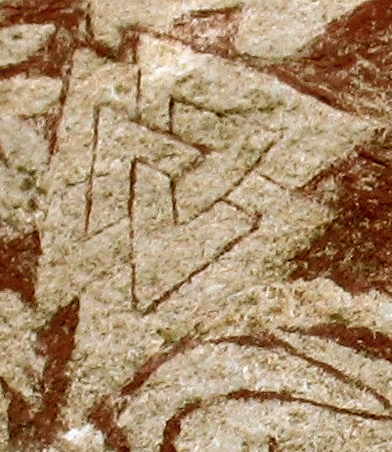
\includegraphics[width=2.5cm]{images/Lecture 19/ValknutStoraHammars.png}\]

Another version of the valknut called the unicursal valknut is not topologically equivalent to the Borromean link:
 it is a knot and ambient isotopic to
 the trefoil. It is the current symbol of the German Football
 Association.
 \[
\includegraphics[width=2.5cm]{images/Lecture 19/DFB_Logo.png}\]
\end{rem}
\begin{defn}
    A link is a finite collection of circles smoothly embedded in $\R^3$: 
    \begin{equation}
        \coprod_{i=1}^k S^1 \hookrightarrow \R^3
    \end{equation}
\end{defn}
In which smoothness is to exclude some pathological situations. For instance the following one
 \[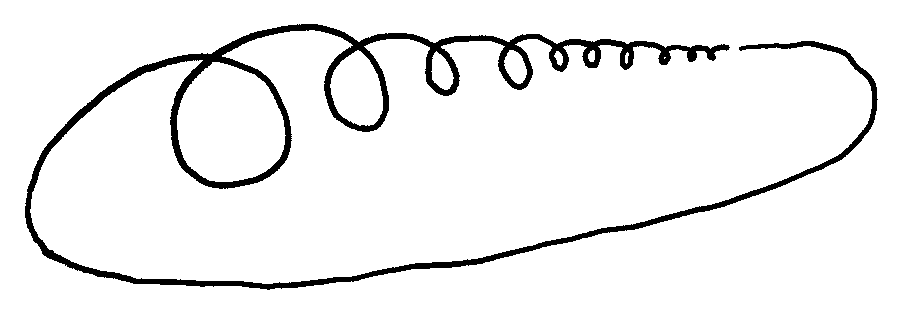
\includegraphics[width=6.6cm]{images/Lecture 19/pathological.png}\]
 This is pathological because it should be intuitively be equivalent to the unknot and to show this we would need 
 infinitely many Reidemeister moves of type 1 (see \ref{moves}) to deform it to the unknot. 
 However, the fundamental theorem of knot theory \ref{ReidemeisterTHM}
 manages to prove that two knots are equal if one can be deformed into the other with \emph{finitely} many 
 Reidemeister moves.
\begin{defn}
    A knot is a link with one component ($k=1$).
\end{defn}

\begin{defn}
    Two links $L_1, L_2: \amalg_{i=1}^k S^1 \hookrightarrow \R^3$ are equivalent if there exists an ambient isotopy between them, i.e. $H: \R^3 \times [0,1] \to \R^3$ such that
    \begin{itemize}
        \item $H(-,0) = id$
        \item $\forall t \in [0,1], \; H(-,t)$ is a diffeomorphism
        \item $H(-,1) \circ L_1 = L_2$
    \end{itemize}
\end{defn}

A goal of knot theory is to find an invariant of knots/links, i.e. an assignment
\begin{equation}
    \{\text{knots/links}\} \to \R, \Z[A,A^{-1}],\dots
\end{equation}
such that if two links are equivalent we get the same number, polynomial, $\dots$.

A link invariant is complete if it detects when 2 links are/are not equivalent.

Concretely, we represent links and nots by 2d drawings, these drawings are called \textit{Link diagrams}. Let $L$ be a link and $p:\R^3 \to \R^2$ a projection.
\begin{defn}
    $p(L)$ is regular if 
    \begin{enumerate}
        \item every point has at most 2 preimages in $L$
        \item intersections are transversal
    \end{enumerate}
\end{defn}
\begin{defn}
    A link diagram is a regular $p(L)$ together with over/under information at each crossing. Visually:
     \[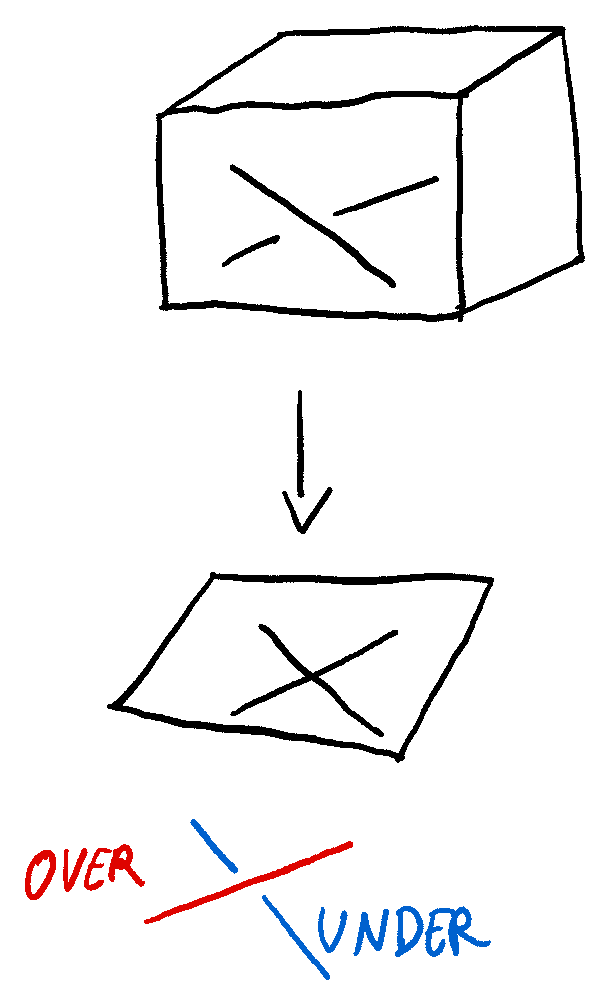
\includegraphics[width=4.6cm]{images/Lecture 19/regularproj.png}\]
\end{defn}
\begin{rem}
    Given a link, we do \textit{not} always get a link diagram $p(L)$, but we can always deform/perturb the embedding $L: \coprod_{i=1}^k S^1 \hookrightarrow \R^3$ by ambient isotopy to $L'$ which gives a link diagram. 
    For instance, the following two projections are irregular: 
     \[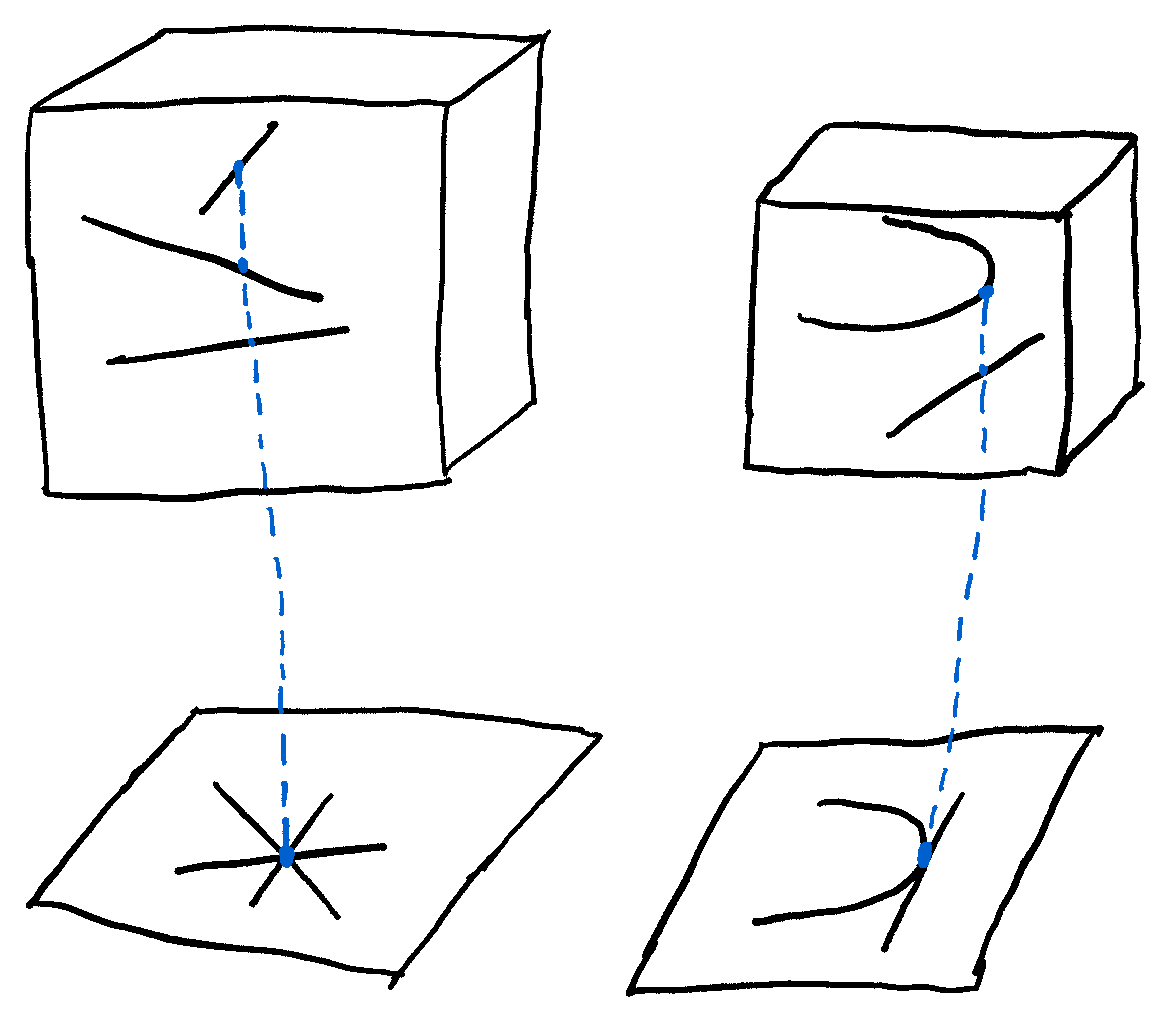
\includegraphics[width=6.6cm]{images/Lecture 19/irregularproj.png}\]
     But such situation could be avoided by moving such links in a reasonable manner via ambient isotopies.
\end{rem}

Our aim is to define a knot/link invariant by defining something on link diagrams. 
In order to do this we introduce Reidemeister moves, which are the following local changes in a link diagram:
\begin{itemize}\label{moves}
    \item (I or R1) \[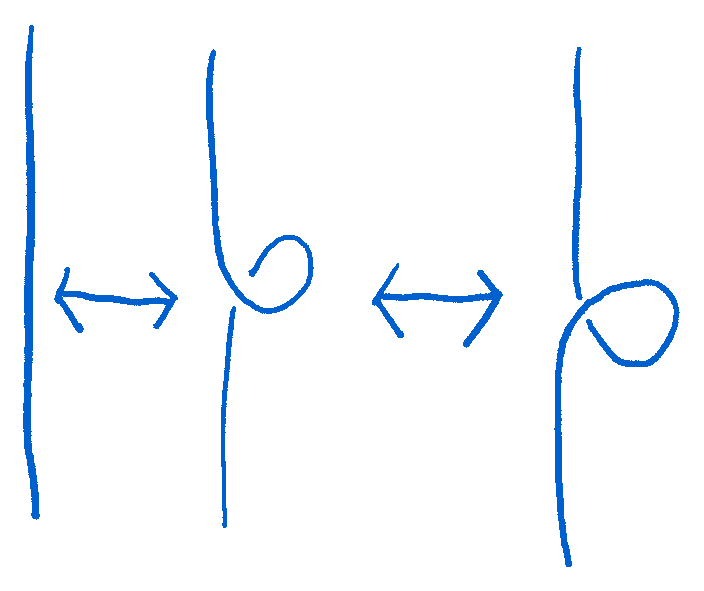
\includegraphics[width=4.6cm]{images/Lecture 19/R1.png}\]
    \item (II or R2) \[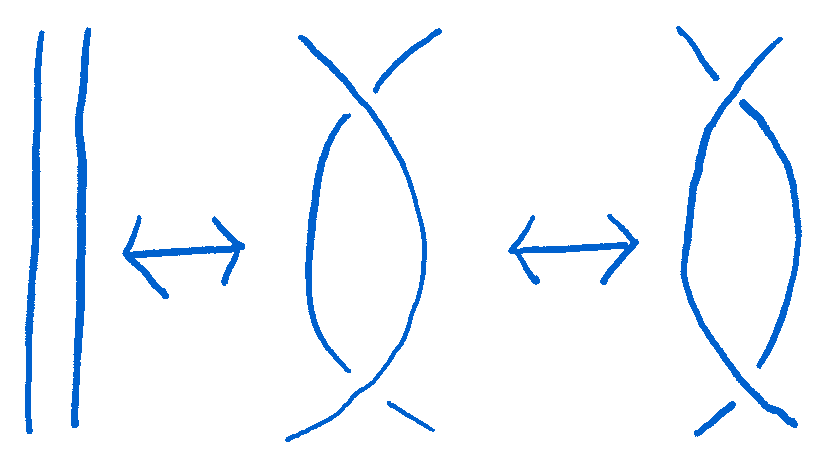
\includegraphics[width=4.6cm]{images/Lecture 19/R2.png}\]
    \item (III or R3) \[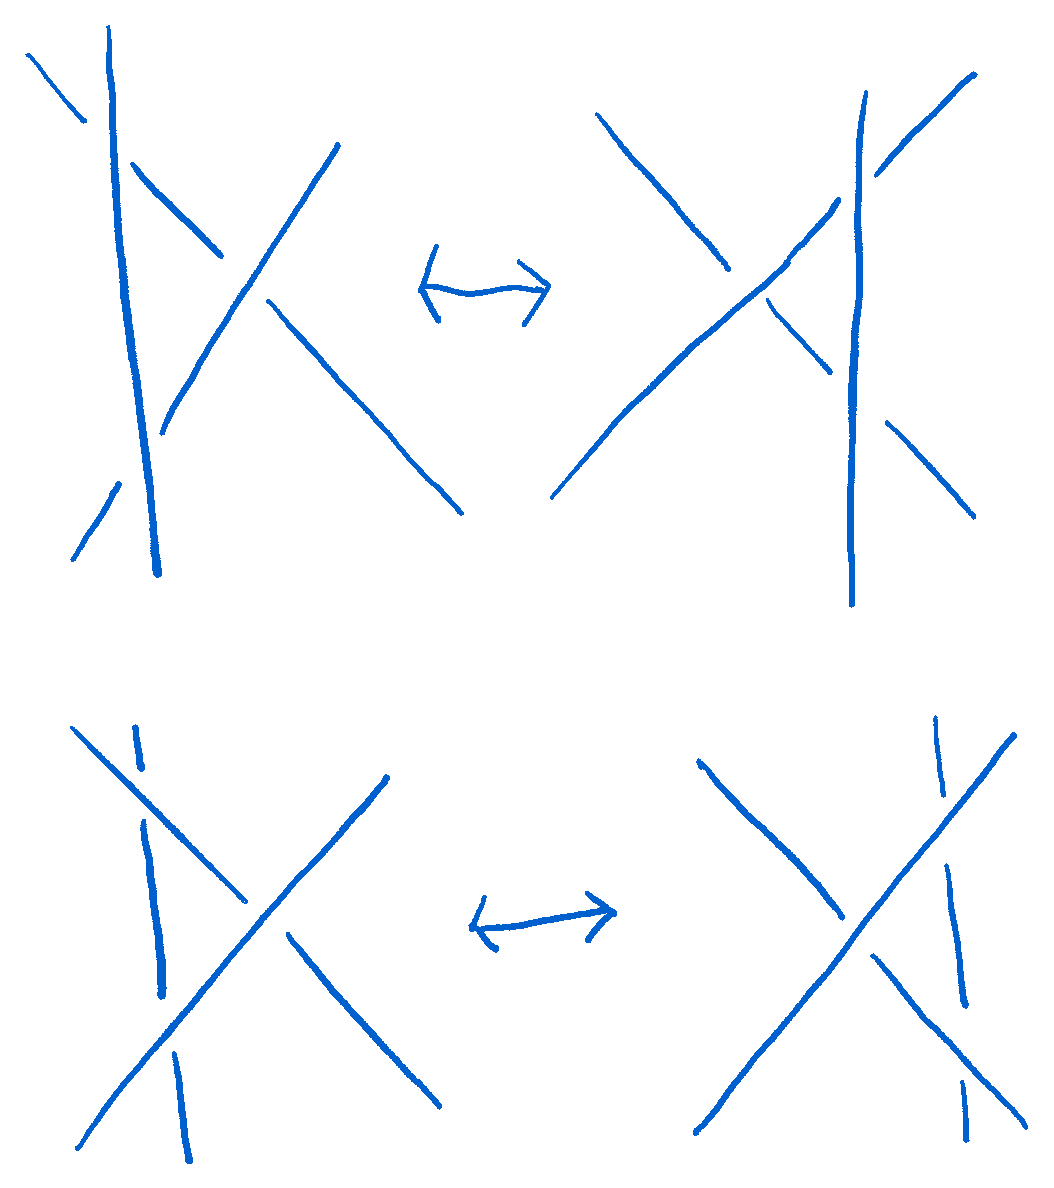
\includegraphics[width=4.6cm]{images/Lecture 19/R3.png}\]
\end{itemize}

\begin{thm}[Reidemeister]\label{ReidemeisterTHM}
    Two links are equivalent if and only if their link diagrams are the same up to finitely many Reidemeister
     moves and isotopies in $\R^2$. 
\end{thm}
This theorem is very important because it tells us that the link diagrams have all the information of the
 equivalence class of the link, so to determine (in)equivalence we can work with link diagrams.

A first knot invariant is the "number of tricolorings": we color a link diagram with three colors according to the following rules
\begin{itemize}
    \item each strand is one color
    \item at each crossing either all three strands are the same color, or they're all different.
\end{itemize}
\begin{ex}
    There are always three trivial colorings, the monochromatic ones. For the unknot, these are the only three tricolorings
    \[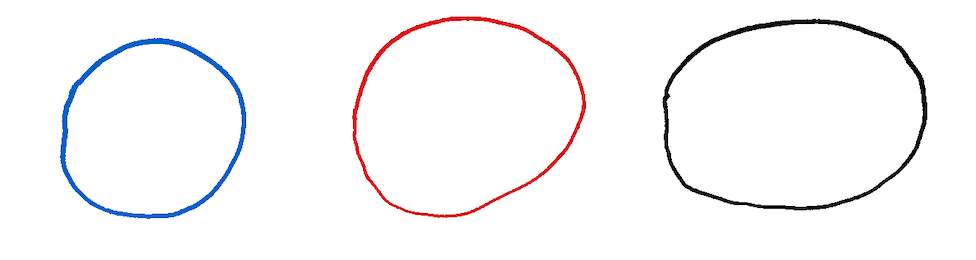
\includegraphics[width=5cm]{images/Lecture 19/Unknotcolors.png}\]
    while the trefoil has an additional one:
   \[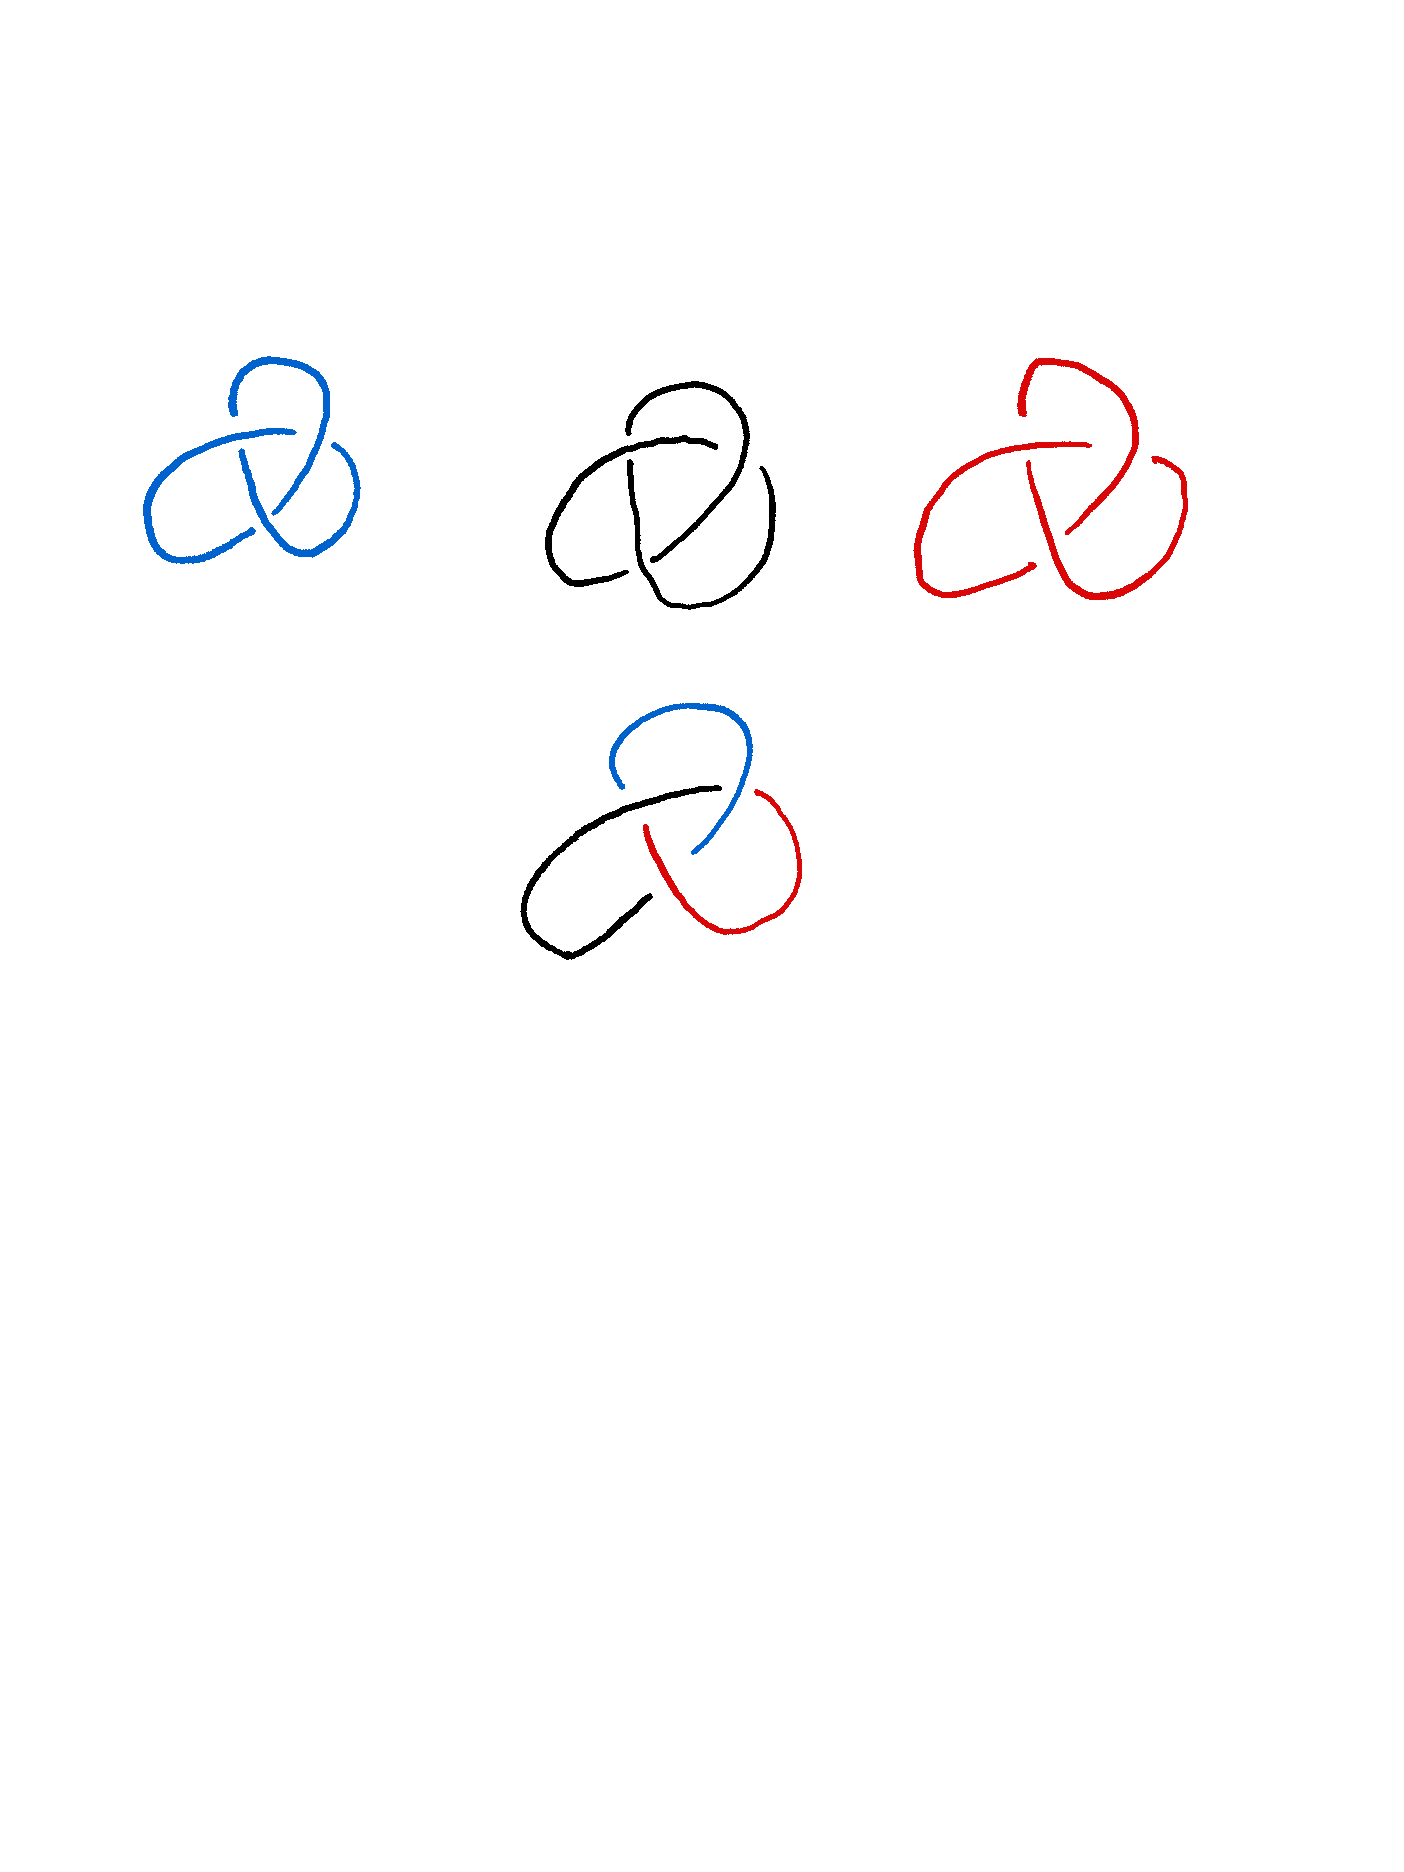
\includegraphics[width=7cm]{images/Lecture 19/Trefoilcolors.png}\]

    This shows that the trefoil knot is \textit{not} equivalent to the unknot.
\end{ex}
In order to prove that this is a knot invariant one should check that it is invariant under Reidemeister moves.

We now finally get to the Jones polynomial, found by Jones in 1984, and this presentation is from Kauffmann in 1987. The motivation for it comes from operator algebras and the braid group representations. 
\begin{defn}
    The Kauffmann bracket of a link diagram $D$ is a Laurent polynomial $\langle D\rangle \in \Z[A,A^{-1}]$ defined by
    \begin{itemize}
        \item $\langle 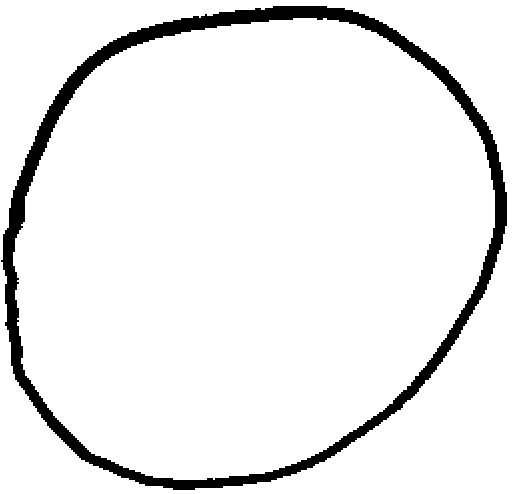
\includegraphics[width=0.4cm]{images/Lecture 19/unknot.png}\rangle = 1$
        \item $\langle 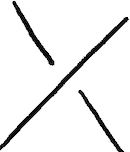
\includegraphics[width=0.4cm]{images/Lecture 19/cross.png}\rangle=A\cdot\langle 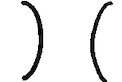
\includegraphics[width=0.4cm]{images/Lecture 19/1Kauffmann.png}\rangle + A^{-1}\cdot\langle 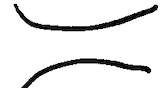
\includegraphics[width=0.4cm]{images/Lecture 19/2Kauffmann.png}\rangle $
        \item $\langle L\cup 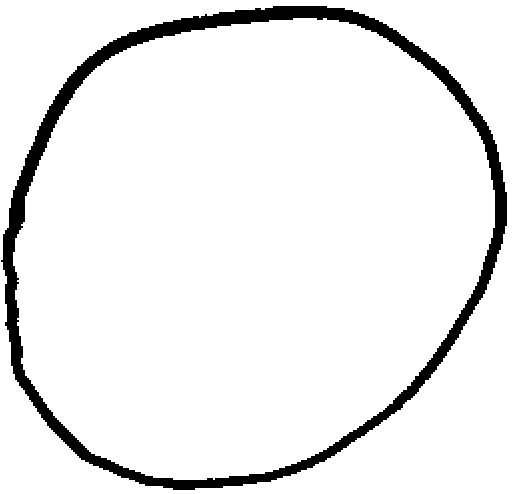
\includegraphics[width=0.4cm]{images/Lecture 19/unknot.png}\rangle=(-A^{2}-A^{-2})\langle L\rangle$
    \end{itemize}
\end{defn}
\begin{ex}
   $$\langle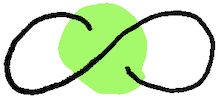
\includegraphics[width=0.7cm]{images/Lecture 19/ooHighlighted.png}\rangle= A\cdot\langle 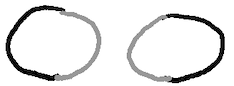
\includegraphics[width=0.7cm]{images/Lecture 19/oo1Kauffmann.png}\rangle + A^{-1}\cdot\langle 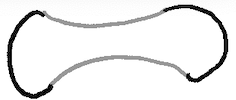
\includegraphics[width=0.7cm]{images/Lecture 19/oo2Kauffmann.png}\rangle =$$
   $$=A(-A^{2}-A^{-2})\langle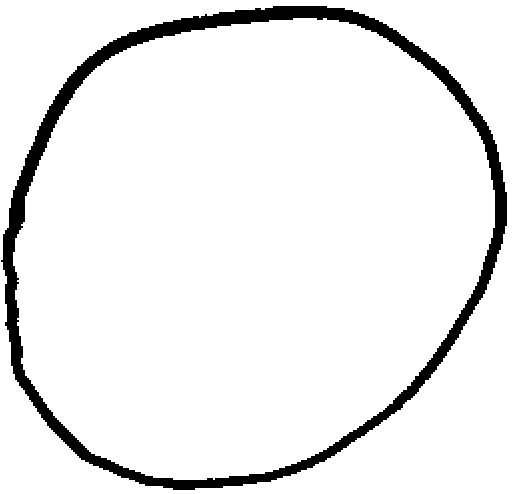
\includegraphics[width=0.4cm]{images/Lecture 19/unknot.png}\rangle + A^{-1}\langle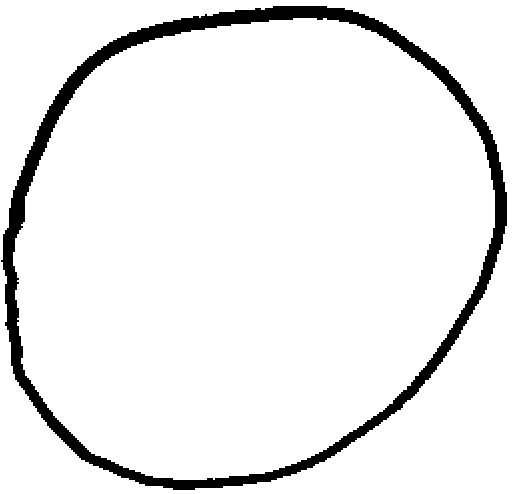
\includegraphics[width=0.4cm]{images/Lecture 19/unknot.png}\rangle=$$
   $$=-A^3-A^{-1}+A^{-1}=-A^3$$
   There is an issue:
   $$\langle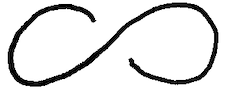
\includegraphics[width=0.7cm]{images/Lecture 19/oo.png}\rangle=\langle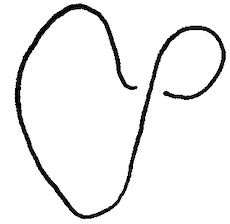
\includegraphics[width=0.55cm]{images/Lecture 19/Laststepkauffmann.png}\rangle$$
   and the last image is equivalent to the unknot, with an application of the first Reidemeister move, but
   $$\langle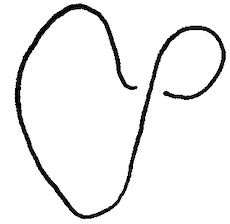
\includegraphics[width=0.55cm]{images/Lecture 19/Laststepkauffmann.png}\rangle=A^3$$
   and 
   $$\langle 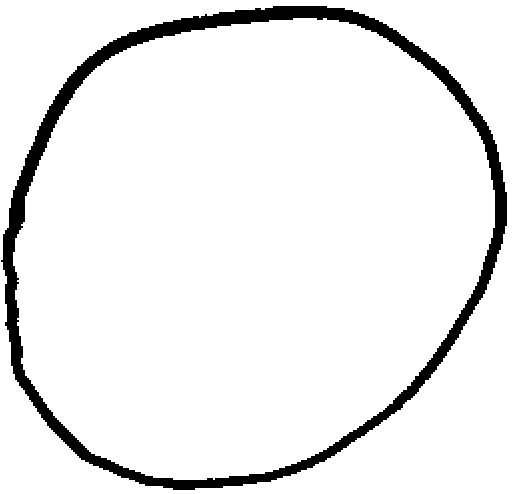
\includegraphics[width=0.4cm]{images/Lecture 19/unknot.png}\rangle = 1$$
   \end{ex}
This shows that the Kauffmann bracket is \textit{not} a knot invariant, in particular it is not invariant under R1. It \textit{is} however invariant under R2 and R3, in fact the coefficients in the definition of the bracket are exactly the ones that preserve R2 and R3.

From now on: links are oriented, meaning $S^1$ comes with an orientation. So we can talk about oriented link invariants, for which we have oriented Reidemeister moves. 

Now we would like to fix the problem with the Kauffmann bracket. 
\begin{defn}
    The sign of a crossing is 
    %DRAWING
\end{defn}
\begin{defn}
    The writhe of an oriented link diagram $D$ is the sum of the signs of the crossings:
    \begin{equation}
        w(D) = \sum_{c \text{ crossing in } D} \sign(c)
    \end{equation}
\end{defn}

\begin{lem}
    The writhe is also invariant under R2 and R3, and changes under R1 as ...
    %DRAWING
\end{lem}

\begin{defn}
    For any link $L$, define $\chi (L) = (-A^3)^{-w(p(L))} \langle p(L)\rangle \in \Z[A^{-1},A]$
\end{defn}
\begin{thm}
    This is a link invariant.
\end{thm}

\begin{ex}
    Hopf link vs two detached links
    %DRAWING
\end{ex}

\begin{defn}
    For any unoriented link $L$, the Jones polynomial of $L$ is 
    \begin{equation}
        V(L) = \chi(L)|_{A=t^{1/4}} \in \Z[t^{-1/2},t^{1/2}]
    \end{equation}
\end{defn}

\begin{ex}
    trefoil %TODO complete

    $V(D) = t+t^3-t^4$
\end{ex}

% -------------------------------------------------------------
% ---------------------- LECTURE 20 24/1 ----------------------
% -------------------------------------------------------------

Observe
\begin{itemize}
    \item $V(unknot) = 1$
    \item skain relation: if $L_+, L_-, L_0$ are the same link except for at one crossing, according to the following picture
    %DRAWING

    then 
    \begin{equation}
        t^{-1}V(L_+) -tV(L_-) + (t^{-1/2} - t^{1/2}) V(L_0) = 0
    \end{equation}
\end{itemize}

Explanation of problem of the Kauffmann bracket with R1:
\begin{defn}[Alternative]
    A framed link is (a link together with a nonvanishing normal vector field as before) the image of a smooth embedding of $\coprod_{i=1}^k S^1 \times [0,1] \hookrightarrow \R^3$.
\end{defn}
\begin{rem}
    This can be projected onto $\R^2$ such that annuli are "flat", this is the "blackboard framing" from previously.
\end{rem}
\begin{ex}
    We can give two framings on the unknot which are not equivalent:
    %DRAWING
\end{ex}
\begin{thm}
    $L,L'$ framed links, $D,D'$ diagrams thereof using blackboard framings. Then $L \sim L'$ (isotopy equivalence with framing) if and only if $D$ is related to $D'$ via R2, R3 and the modification of R1 given by
    %DRAWING
\end{thm}
\begin{thm}
    The Kauffmann bracket is a framed link invariant.
\end{thm}
Recall we had $\Tang_1^{or,fr}(\cat) \to \cat$ where \cat is a ribbon category. Now, fix a $V \in \cat$, we get an injection $\Link^{or,fr} \hookrightarrow \Tang_1^{or,fr}(\cat)$ in which we decorate each strand (component) by $V$. The goal is then to find a specific ribbon category \cat such that we get back the Jones polynomial. We'll find $\cat = U_q\sl_2 -Mod^{f.d.}$.


\subsection{Making \texorpdfstring{$A-\Mod^{f.d.}$}{A-Mod f.d.} into a ribbon category} % (fold)
\label{ssub:making_}

%Back to algebra: How to get a ribbon category?
We now want to add additional structures on an algebra $A$ in such a way that $A-\Mod^{f.d.}$ becomes a ribbon category.
%why do we want to do this?
We therefore need $A-\Mod^{f.d.}$ to have the following structures:
\begin{itemize}
    \item monoidal structure,
    \item existence of (right) duals (right rigidity),
    \item braiding,
    \item pivotal structure,
    \item twist,
\end{itemize}
which we gradually construct in this order. 

\subsection*{Monoidal structure} % (fold)

In order to do this, we will need additional structures on $A$, starting with the following.
\begin{defn}
    A Hopf algebra in a braided strict monoidal category \cat is 
    \begin{itemize}
        \item a bialgebra $(H,\mu,\eta,\Delta,\epsilon)$, in which we represent all these maps as the following drawings
        %DRAWING

        These maps should satisfy
        \begin{equation}
            (\mu \otimes \mu) \circ( id \otimes \beta \otimes id) \circ (\Delta \otimes \Delta) = \Delta \circ \mu
        \end{equation}
        and
        %TODO complete
        \item antipode map $S: H \to H$ depicted as 
        %DRAWING

        satisfying
        %DRAWING
    \end{itemize}
\end{defn}
\begin{ex}
    \item Take $H = k[G]$, 
    \begin{equation}
        \begin{matrix}
            \mu(g,h) = gh\quad & \eta(1) = 1\quad & \\
            \Delta(g) = g \otimes g\quad & \epsilon(g) = 1\quad & s(g)  = g^{-1} 
        \end{matrix}
    \end{equation}
    \item for Lie algebra \g, let $U\g$ be its universal enveloping algebra, which we will define shortly. We then have
    \begin{equation}
        \Rep^{f.d.} G \simeq U\g-\Mod^{f.d.}
    \end{equation}
    we will then "deform" this in one of the exercises.
\end{ex}

Recall that a Lie algebra is defined as follows.
\begin{defn}
    A Lie algebra is a vector space with a bilinear map $[-,-]: \g \otimes \g \to \g$, sending $x \otimes y \mapsto [x,y]$, called the Lie bracket, satisfying:
    \begin{itemize}
        \item anticommutativity: $[x,x]=0$ or $[x,y] = -[y,x]$
        \item Jacobi identity: $[x,[y,z]] + [y,[z,x]] + [z,[x,y]] = 0$
    \end{itemize}
    A homomorphism of Lie algebras $\g, \mathfrak h$ is a linear map $\phi: \g \to \mathfrak h$ such that $\phi([x,y]_\g) = [\phi(x), \phi(y)]_{\mathfrak h}$.
\end{defn}
\begin{ex}
\hfill
    \begin{enumerate}
        \item $\g = \End(V) = \gl_V$, with bracket given by the commutator $[f,g] = f \circ g - g \circ f$. There is also a sub Lie algebra $\sl_V:=\{f \in \gl_V : \tr f = 0\}$.

        If for example we take $V = \R^2$ we have $\gl_2 = \Mat_{2,2}$ and $\sl_2 = \{A \in \Mat_{2,2}: \tr A = 0\}$.
        \item Let $A$ be an associative algebra, then if we take the underlying vector space, with bracket given by the commutator, we get a Lie algebra. In other words, there is a forgetful functor:
        \begin{equation}
            \Alg \to \Lie
        \end{equation}
        and its left adjoint is the concept of universal enveloping algebra which we will see more explicitly later on.
        \item %TODO complete
        \item smooth vector fields on a smooth manifold: $\mathfrak{X} = \Der(\C^\infty(M))$ %TODO weird letter
    \end{enumerate}
\end{ex}
Outlook: in physics we like to look at Lie groups, a smooth manifold with a group structure (i.e. a group object in the category of smooth manifolds). Since it's a manifold, we can look at its tangent space. The Lie algebra $\g$ of $G$ is defined as $T_e G$. %left invariant vector fields....

Now, fix \g a Lie algebra.
\begin{defn}
    The tensor algebra of \g is the (graded) algebra given by:
    \begin{equation}
        T(\g) := \bigoplus_{n=0}^\infty \g^{\otimes n}
    \end{equation}
    with $\g^{\otimes n} \otimes \g^{\otimes k} \to \g^{\otimes(n+k)}$.

    There is a 2 sided ideal $I(\g) \subset T(\g)$ generated by $\langle x \otimes y - y \otimes x - [x,y] \rangle$. We can then define the universal enveloping algebra of \g:
    \begin{equation}
        U\g := T(\g)/I(\g)
    \end{equation}
\end{defn}
The universal enveloping algebra has the universal property that given an algebra $A$ and a Lie algebra map $\g \to A$ there is a unique map $U \g \to A$ making the following diagram commute
\begin{equation}
    \begin{tikzcd}[nodes in empty cells=true]
        \g \ar[dr]\ar[r] & U\g \ar[d, dashed] \\
        & A
    \end{tikzcd}
\end{equation}

\begin{clm}
    $U\g$ is a Hopf algebra, with coalgebra structure given by:
    \begin{itemize}
        \item $\Delta: U\g \to U\g \otimes U\g$ %TODO complete
        \item $\epsilon: U\g  \to k$
        \item $S: U\g \to U\g$
    \end{itemize}
\end{clm}
In general, we'll now see that if $A$ is a Hopf algebra, then $A-\Mod^{f.d.}$ is a monoidal category with duals.

\begin{thm}
    Let $(A,\mu,\eta)$ be a unital associative algebra and $\Delta:A \to A \otimes A, \epsilon:A \to k$ linear maps. Then $(A,\mu,\eta, \Delta, \epsilon)$ is a bialgebra if and only if $(A-\Mod, \otimes , (k,\epsilon))$ is monoidal.
\end{thm}
\begin{itemize}
    \item Let $M,N$ be $A-$modules, then the vector space $M\otimes N$ is an $A-$module via 
    \begin{equation}
        \begin{tikzcd}
            A \ar[r, "\Delta"] & A \otimes A \ar[r] & \End(M) \otimes \End(N) \ar[r] & \End(M \otimes N)
        \end{tikzcd}
    \end{equation}
    \item $(k,\epsilon)$ is an $A-$module via
    \begin{equation}
        A \xrightarrow{\epsilon} \End(k) \cong k
    \end{equation}
    \item associators and unitors are those from $\Vect$.
\end{itemize}

\subsection*{Rigidity} % (fold)

%Schweigert cor 2.5.17 says kind of the opposite, I ALWAYS have a right dual and only have a left dual if S is invertible
\begin{prop}\label{prop:Hopf2}
    Let $H$ be a Hopf algebra and $M$ an $H-$module, then $M^\vee:=\Hom(M,k)$ has an $H$ action via the transpose of $S$, i.e. given $\phi \in \Hom(M,k),\,a \in H$ we get $a \cdot \phi \in \Hom(M,k)$ given by
    \begin{equation}\label{eq:dual_mod_struct}
        (a \cdot \phi) (m):= \phi(s(a) \cdot m)
    \end{equation}
    This is a left dual if $M$ is finite dimensional.
    Now, if $S$ is invertible, ${}^\vee M = \Hom(M,k)$ with $(a \cdot \phi)(m) := \phi(s^{-1}(a)\cdot m)$ is a right dual if $M$ is finite dimensional.
\end{prop}

\begin{cor}
    If $H$ is a Hopf algebra with $S$ invertible, then $H-\Mod^{f.d.}$ is rigid monoidal.
\end{cor}
\begin{proof}[Idea of proof of Proposition \ref{prop:Hopf2}]
    Check that $ev_M, coev_M$ exhibiting dual in $\Vect$ are $H-$module maps.
\end{proof}

% Outlook: To get a ribbon category we need:
% \begin{itemize}
%     \item braiding
%     \item pivotal structure
%     \item twist
% \end{itemize}

% -------------------------------------------------------------
% ---------------------- LECTURE 21 29/1 ----------------------
% -------------------------------------------------------------

\subsection*{Braiding} 
Recall: we want a ribbon category and we had a Hopf algebra, so we had a monoidal category with duals.

We're now using \cite{SchwHopfQuantumTFT} as a reference.

\begin{defn}
    A quasi-triangular structure on a bi/Hopf algebra is a "universal $R$-matrix", i.e. an invertible element $R \in A \otimes A$ such that $\forall x \in A$ with 
    \begin{equation}
        \begin{tikzcd}
            \Delta^{coop}: A \ar[r, "\Delta"] & A \otimes A \ar[r, "\tau_{A,A}"] & A \otimes A
        \end{tikzcd}
    \end{equation}
    the following are satisfied
    \begin{enumerate}
        \item $\Delta^{coop}(x) R  = R \Delta(x)$, and
        \item In $A^{\otimes 3}$ we have 
        \begin{align}
            (\Delta \otimes id_A)(R) = R_{13} R_{23} 
        \end{align}
        \item 
        \begin{equation}
            (id_A \otimes \Delta)(R) = R_{13} R_{12}
        \end{equation}
        in which $R_{12} = R \otimes 1, R_{23} = 1 \otimes R, R_{13} = (\tau_{A,A} \otimes id_A)(1 \otimes R)$
    \end{enumerate}
\end{defn}

\begin{ex}
    Any cocommutative bi/Hopf algebra has a canonical $R$ matrix, $R = 1\otimes 1$, since the first relation simply becomes $\Delta = \Delta^{coop}$, which is exactly the cocommutativity.
\end{ex}

\begin{prop}[4.2.3. in \cite{SchwHopfQuantumTFT}]
    Let $A$ be a bialgebra. Then a braiding on $A-\Mod^{(f.d.)}$ uniquely determines a quasitriangular structure on $A$ and viceversa. 
    % This is what we're trying to do: add structures on A so that A-Mod has more structure.
\end{prop}

\begin{proof}[Proof strategy: ]
    Given a braiding $\beta$, define the universal $R$ matrix to be
    \begin{equation}
        R:=\tau_{A,A}(\beta_{A,A}(1_A \otimes 1_A))
    \end{equation}
    in which $\tau_{A,A}$ is the flip and $\beta_{A,A}$ is the braiding. Then one can check properties 1. 2. and 3. above. 

    Now, the following is also true:
    \begin{clm}
        Given $R$ as above, the braiding can be recovered as follows: $\beta_{U,V} (u \otimes v) = \tau_{U,V}(R(u \otimes v))$, for arbitrary $U, V \in A-\Mod$.
    \end{clm}
    So this motivates that if we are given a universal $R$ matrix, we should define $\beta$ as such, and one should check that it's actually a braiding.
\end{proof}

We're now using \cite{tingley2015minus} as a reference.
Main example: $U_q\sl_2$, Hopf algebra, not cocommutative but has a universal $R$ matrix. Therefore $U_q\sl_2 - \Mod$ is braided monoidal. We get $U_q\sl_2$ from the cocommutative Hopf algebra $U\sl_2$ by "deforming" it.

$U_q\sl_2$ is a $\C(q)$-algebra generators $E,F,K,K^{-1}$ with relations:
\begin{align*}
    KK^{-1} &= K^{-1}K = 1 \\
    KEK^{-1} &= q^2 E \\
    KFK^{-1} &= q^{-2}F \\
    [E,F] &= \frac{K - K^{-1}}{q - q^{-1}}
\end{align*}
We have an important 2 dimensional module ("representation") for $U_q\sl_2$: $V_1 \cong \C^2$ with basis $v_1, v_{-1}$. Now, how does $U_q\sl_2$ act? In this basis we write:
\begin{align*}
    E &=
    \begin{pmatrix}
        0 & 1 \\
        0 & 0 
    \end{pmatrix} \\
    F &= 
    \begin{pmatrix}
        0 & 0 \\
        1 & 0 
    \end{pmatrix} \\
    K &= 
    \begin{pmatrix}
        q & 0 \\
        0 & q^{-1} 
    \end{pmatrix} 
\end{align*}

We also claimed there was a Hopf algebra structure, which we now make explicit. The comultiplication is given by
\begin{align*}
    \Delta(E) &= 1\otimes E + E \otimes K \\
    \Delta(F) &= K^{-1} \otimes F + F \otimes 1 \\
    \Delta(K) &= K \otimes K \\
    \Delta(K^{-1}) &= K^{-1} \otimes K^{-1}
\end{align*}
the counit map:
\begin{align*}
    \epsilon(E) &= \epsilon(F) = 0 \\
    \epsilon(K) &= \epsilon(K^{-1}) = 1
\end{align*}
and we should check that these satisfy the required relations. In addition we need the antipode map:
\begin{align*}
    S(E) &= -EK^{-1}\\
    S(F) &= -KF \\
    S(K) &= K^{-1} \\
    S(K^{-1}) &= K
\end{align*}
We then get the monoidal category $U_q \sl_2-\Mod$. If $U,V$ are objects in $U_q \sl_2-\Mod$, then so is $U\otimes V$ in which we have
\begin{equation}
    E(u \otimes v) = E_U \otimes K_V + U \otimes E_V
\end{equation}
It is also braided... %TODO complete

From $S$ we get the dual of $V_1$: as vector space $V_1^\vee = \Hom(V_1, \C)$, in which $\hat v_1, \hat v_{-1}$ is the dual basis. This has a $U_q \sl_2-\Mod$ structure given by Equation \ref{eq:dual_mod_struct}.

Up to now we therefore get the following correspondence between the structures on $A$ and those on $A-\Mod^{f.d.}$:
\begin{center}
\begin{tabular}{ccc}
bialgebra &$\leftrightarrow$& monoidal \\
Hopf algebra &$\leftrightarrow$& right rigid \\
Hopf with $S$ invertible &$\leftrightarrow$& rigid \\
quasi-triangular &$\leftrightarrow$& braiding 
\end{tabular}
\end{center}


% -------------------------------------------------------------
% ---------------------- LECTURE 22 5/2 -----------------------
% -------------------------------------------------------------

%Tingley a minus sign... https://arxiv.org/abs/1002.0555
%recollection...

Let's make explicit the dual representation to $V_1$, $V_1^\vee = \Hom(V, \C) = \langle \hat v_1, \hat v_{-1}\rangle$, where $\hat v_1$ and $\hat v_{-1}$ are the dual basis.

Recall that we had the \textit{decorated} tangle category. Let's take $\cat = U_q\sl_2 - \Mod^{f.d.}$ and let $V=V_1$ the representation above. In particular we work with "$\Tang_1^{fr,or}(V_1)$"$\subset \Tang_1^{fr,or}(\cat)$ in which we decorate everything with just $V_1$.

\begin{rem}
    \begin{itemize}
        \item $A = q^{-1/2}$
        \item slightly different normalization: $F(unknot) = -q -q^{-1}$.
        \item What about the third relation of the Kauffmann bracket? It follows from monoidality!
    \end{itemize}
\end{rem}

\section{Outlook: How to get a 3D TFT?} % (fold)
\label{sec:outlook_how_to_get_a_3d_tft_}

\subsection{From knots to 3 manifolds: surgery} % (fold)
\label{sub:from_knots_to_3_manifolds_surgery}

Given: a framed link $L\subset S^3$ (so far $L\subset\R^3$ but we now embed that into $S^3$) with $m$ components $L= L_1 \cup \dots \cup L_m$ with $L_i \cong S^1$. Now:
\begin{itemize}
    \item Choose closed tubular neighborhood $U \subset S^3$ of link $L$ such that $U = U_1 \amalg \dots \amalg U_m$:
        \begin{equation}
            \begin{tikzcd}
                L_i \ar[r, phantom, "\cong"]\ar[d, phantom, "\cap"] & S^1 \times \{0\} \\
                U_i \ar[r, "\phi"', "\cong"] & S^1 \times D^2
            \end{tikzcd}
        \end{equation}
        framing of $L_i \cong$ constant normal vector field on $S^1\times\{0\} \hookrightarrow S^1 \times D^2$.
        Could also have the nonconstant framing, that turns around once.
    \item $\de(S^3 \setminus \operatorname{int}(U_1 \amalg\dots\amalg U_m)) = \de(U_1 \amalg\dots\amalg U_n) \cong S^1 \times S^1 \amalg \dots\amalg S^1\times S^1$, $m$ tori. Now glue in solid tori $D^2\times S^1$ (note that the order here matters) using identity as gluing map to get a closed connected 3 manifold. 
\end{itemize}

\begin{exercise}
    Try unknot with trivial framing.
\end{exercise}

% -------------------------------------------------------------
% ---------------------- LECTURE 23 7/2 -----------------------
% -------------------------------------------------------------

Objective: 3d tqft.
Surgery.

%TODO cite bakalov kirillov lectures on tensor categories and modular functors
Start with a link $L\subset S^3$ with $L= L_1 \amalg \dots \amalg L_m$ with $L_i \cong S^1$. We take a tubular neighborhood of $L$, $U = U_1 \amalg \dots \amalg U_m$ with $U_i \cong S^1 \times D^2$. Let $T := S^1\times D^2$, the full torus, and let $\phi: U_i \xrightarrow{\cong} T$. Now we can define
\begin{equation}
    M_{L,\phi} :=(S^3 \setminus \operatorname{int}(\bigcup_{i=1}^m U_i)) \coprod_{\phi} T^m
\end{equation}
surgery of $S^3$ along $L$ via $\phi$.
However, the result depends on the choice of $\phi$ and we'll see that it corresponds to a choice of framing on the knot.

If $L$ is framed and oriented, we can choose a $\phi$ as follows: let's restric to one component $L_i$. We then have $\de U_i \cong S^1 \times S^1$ and the framing determines a "cycle" of $S^1 \times S^1$ as can be seen in the drawing. In particular if the framing winds around $k$ times then we get a cycle that winds around once in the longitudinal direction and $k$ times in the other direction. This determines a diffeomorphism on the torus up to to isotopy, called the "Dehn twist". 
% DRAWING
We then compose with $swap: S^1 \times S^1 \to S^1 \times S^1$:

\begin{equation}
    \phi_i: 
    \begin{tikzcd}
        T \ar[r] & T \\
        \alpha_i \ar[r, mapsto] & -\beta_i \\
        \beta_i \ar[r, mapsto] & \alpha_i \\
    \end{tikzcd}
\end{equation}

% is this the same diagram?
% https://q.uiver.app/#q=WzAsNSxbMSwwLCIgIFxcYWxwaGFfaSAiXSxbMSwyLCIgXFxiZXRhX2kiXSxbMiwwLCItXFxiZXRhX2kiXSxbMiwyLCJcXGFscGhhX2kiXSxbMCwxLCJcXHBoaV9pIl0sWzAsMl0sWzEsM11d
% \[\begin{tikzcd}[cramped]
%   & {  \alpha_i } & {-\beta_i} \\
%   {\phi_i} \\
%   & { \beta_i} & {\alpha_i}
%   \arrow[from=1-2, to=1-3]
%   \arrow[from=3-2, to=3-3]
% \end{tikzcd}\]

In short, via $\phi_i$ the induced framing on $S^1 \times \{0\}$ is a constant normal framing. So framing on $L$ determines/encodes/records the diffeomorphism $\phi$.

Notation: $L$ framed $M_L:= M_{L,\phi}$ with $\phi$ as above.
\begin{ex}
\hfill
    \begin{itemize}
        \item $L= \emptyset$, we then get $M_L = S^3$,
        \item $L= unknot$ with constant framing:
        \begin{equation}
            \de(S^3 \setminus \operatorname{int} T) \cong S^1 \times S^1
        \end{equation}
        Now, as a warmup let's see how $T \coprod_{\phi'} T = S^2$:
        %DRAWING

        \noindent Now, $(S^3\setminus \operatorname{int} T)  \coprod_{\phi'} T$...

        We then have a well defined projection $M_L \to S^1$ and the fibers of this map are $S^2 = D^2 \coprod_{\de D^2} D^2$. In particular, the bundle is trivial:
        \begin{fct}
            $M_L \cong S^1 \times S^2$.
        \end{fct}
        \item $L = unknot$ with framing with one twist, we get $M_L = S^3$
    \end{itemize}
\end{ex}
The last example is important because it shows that multiple framed links can give the same 3 manifold. However we have the following result:
\begin{thm}
    [Lickorice-Wallace]
    Any connected closed oriented 3-manifold can be obtained as $M_L$ for some framed link $L$ in $S^3$ via surgery.
\end{thm}
We can therefore try to define a manifold invariant by defining it on framed links, but we have to make sure that links that give the same 3 manifold have the same invariant.

\begin{thm}
    [Kirby's theorem]
    $M_L \cong M_{L'}$ if and only if $L'$ is obtained from $L$ by a finite sequence of isotopies and \textit{Kirby moves} which are as follows:
\[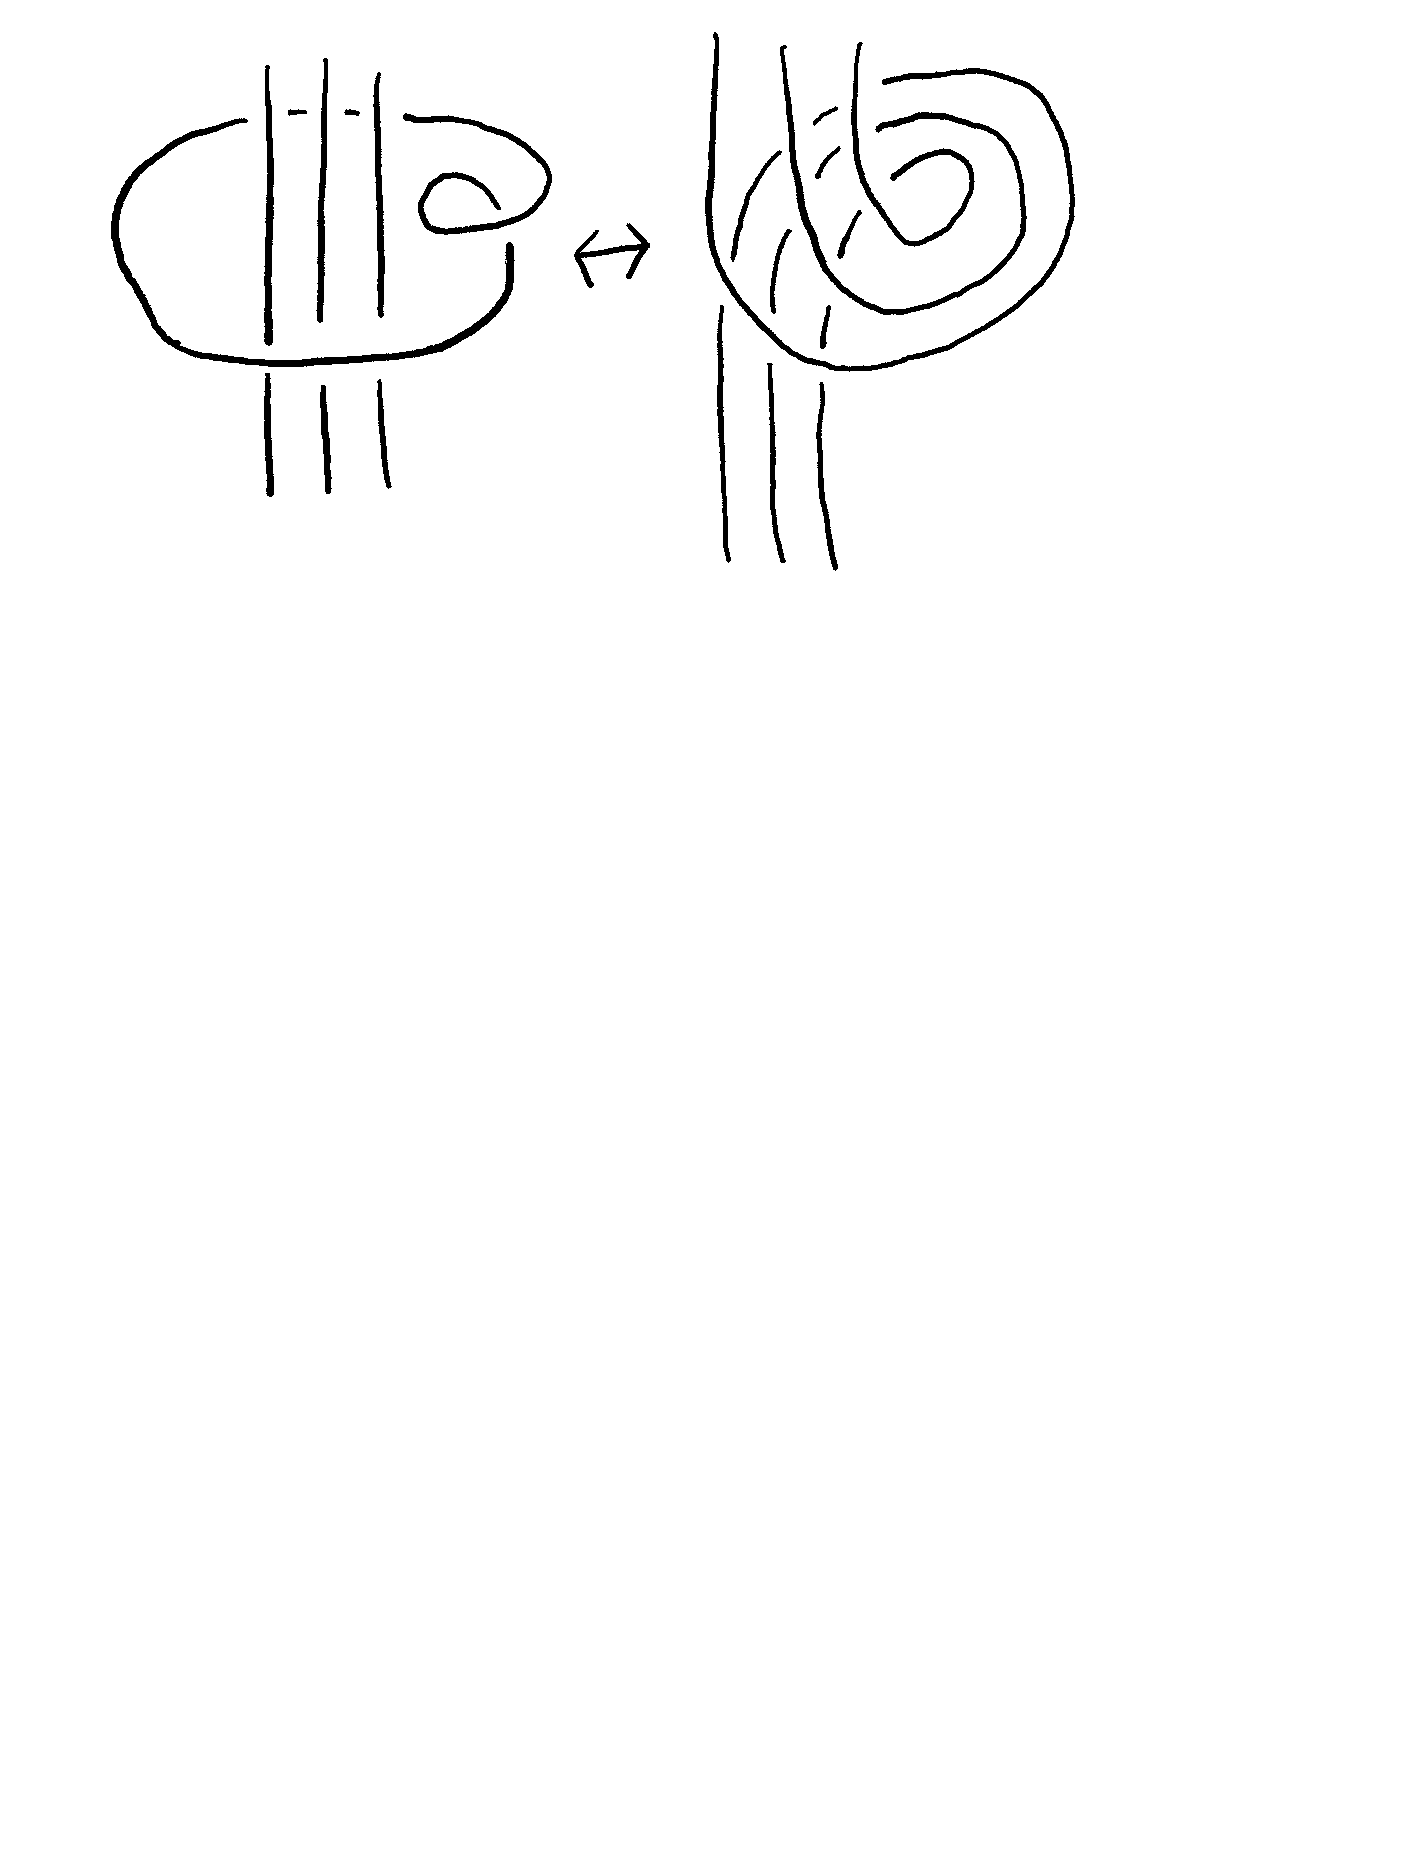
\includegraphics[width=6cm]{images/Final Lecture/KIRBY.png}\]
\end{thm}

We can now get a Reshetikin-Turaev invariant, see for details \cite{KasselRossoTuraev97}. %TODO TBD

\begin{rem}
If $L_1$ and $L_2$ are not linked, then $M_{L_{1}\amalg L_{2}}=M_{L_1}\#M_{L_2}$
Moreover, $\tau(M_{L_1}\#M_{L_2})=c\dot \tau(M_{L_1})\cdot\tau(M_{L_2})$ where $c$ is a constant depending on the
modular tensor category
\end{rem}
We can give a \textbf{rough sketch} of the following theorem
\begin{thm}[Turaev]
For any modular tensor category we have an oriented 3d TFT which generalizes the Reshetikin-Turaev invariants.
\end{thm}
Modular tensor categories are hard to define. The following definition is from \cite{RunkelALG}.
\begin{defn}[Modular Tensor Category]
A modular tensor category is a strict $k$-linear\footnote{I.e. $\Vect_{k}$-enriched.} abelian semisimple ribbon category
such that the index set is finite, every simple object is absolutely simple, and for which the $s$-matrix 
$s=(s_{i,j})_{i,j\in I}$ with entries 
$$s_{i,j}:=s_{U_{i},U_{j}}=\operatorname{tr}(c_{U_{i},U_{j}}\circ c_{U_{j},U_{i}})$$
is non-degenerate. An element $\mathcal{D}\in k$ is called rank of a modular tensor category $\cat$ if 
$$\mathcal{D}^2=\Sigma_{i\in I}(dim (U_i))^2$$
Given a simple object $U_i\in \cat$, also $U_{i}^{\vee}$ is simple.
\end{defn}
See \ref{AbelianCat} for the definition of abelian category.
\begin{rem}
    In the original definition by Turaev (\cite{Turaev+2016}, \cite{TuraevMODTENSOR}) some conditions were
     weaker. It was enriched over Mod$_R$, with $R$ being a commutative ring instead of a field $k$,
     semisimplicity was replaced by the weaker dominance property and instead of it being abelian, it was
     just additive.
\end{rem}
\begin{ex}
\begin{itemize} \hfill
\item $\Vect_k$
\item $U_{q}sl_2-mod^{\operatorname{fd}}$ for $q$ a root of unity
\end{itemize}
\end{ex}
\begin{defn}[Simple object]
An object $U\in\cat$ where $\cat$ is an abelian category is simple if it has no non-trivial subobjects, i.e. 
any injection $V\hookrightarrow U$ is either the 0 object or an isomorphism.
\end{defn}
\begin{defn}[Semisimple object]
An object $U\in\cat$ where $\cat$ is an abelian category is semisimple if it is isomorphic to a direct sum of 
simple objects.
\end{defn}
\begin{defn}[Semisimple category]
An abelian category is semisimple if it only has semisimple objects.
\end{defn}
\begin{defn}[Absolutely simple object]
    An object $U\in\cat$ where $\cat$ is an abelian $k$-linear category is called absolutely simple if and only if 
    $\Hom(V,V)=k \id_V$. If $\cat$ is semisimple and $k$ algebraically closed, then this is equivalent to a simple 
    object.
\end{defn}